\documentclass[a4paper, openany]{memoir}

\usepackage[utf8]{inputenc}
\usepackage[T1]{fontenc} 
\usepackage[english]{babel}

\usepackage{fancyhdr}
\usepackage{float}

\usepackage{amsmath}
\usepackage{amsthm}
\usepackage{amssymb}
\usepackage{enumitem}
\usepackage{multicol}
\usepackage[bookmarksopen=true,bookmarksopenlevel=2]{hyperref}
\usepackage{tikz}
\usepackage{indentfirst}

\pagestyle{fancy}
\fancyhf{}
\fancyhead[LE]{\leftmark}
\fancyhead[RO]{\rightmark}
\fancyhead[RE, LO]{Data Fundamentals}
\fancyfoot[LE, RO]{\thepage}
\fancyfoot[RE, LO]{Pete Gautam}

\renewcommand{\headrulewidth}{1.5pt}

\chapterstyle{thatcher}
\setcounter{chapter}{2}
\begin{document}
    \chapter{Vectors and Matrices}
    \section{Vector Spaces}
    Vectors are ordered tuples of real numbers
    \[\begin{bmatrix}
        x_1 & x_2 & \dots & x_n
    \end{bmatrix}.\]
    A vector has a fixed dimension $n$- this is the length of the tuple. For example, $\begin{bmatrix}
        5 & 3 & 7
    \end{bmatrix}$ is a vector in $\mathbb{R}^3$.

    We use the following notations to denote sets:
    \begin{itemize}
        \item $\mathbb{R}$- the set of real numbers;
        \item $\mathbb{R}_{\geq 0}$- the set of non-negative real numbers;
        \item $\mathbb{R}^n$- the set of tuples of real numbers, of length $n$;
        \item $\mathbb{R}^{n \times m}$- the set of 2D arrays (i.e. matrices) with $n$ rows and $m$ columns.
        \item $(\mathbb{R}^n, \mathbb{R}^n) \to \mathbb{R}$- an operation that maps two vectors in $\mathbb{R}^n$ to $\mathbb{R}$.
    \end{itemize}
    \subsection{Vector operations}
    The set $\mathbb{R}^n$ is an $n$-dimensional real vector space (i.e. tuples containing $n$ elements). They have the following operations:
    \begin{itemize}
        \item scalar multiplication, i.e. multiplying a vector with a real number. If $\mathbf{x} = \begin{bmatrix}
            x_1 & x_2 & \dots & x_n
        \end{bmatrix}$, then
        \[a \mathbf{x} = \begin{bmatrix}
            ax_1 & ax_2 & \dots & ax_n
        \end{bmatrix}.\]
        It is an operation $(\mathbb{R}, \mathbb{R}^n) \to \mathbb{R}^n$.
        
        \item vector addition, i.e. adding two vectors. If $\mathbf{x} = \begin{bmatrix}
            x_1 & x_2 & \dots & x_n
        \end{bmatrix}$, and $\mathbf{y} = \begin{bmatrix}
            y_1 & y_2 & \dots & y_n
        \end{bmatrix}$, then
        \[\mathbf{x} + \mathbf{y} = \begin{bmatrix}
            x_1 + y_1 & x_2 + y_2 & \dots & x_n + y_n
        \end{bmatrix}.\]
        It is an operation $(\mathbb{R}^n, \mathbb{R}^n) \to \mathbb{R}^n$. Two vectors with different dimensions cannot be added- they live in two different vector spaces.

        \item norm, which measures the length of a vector. It is an operation of the form $\mathbb{R}^n \to \mathbb{R}_{\geq 0}$.
        
        \item inner product, which allows the angles of two vectors to be compared. If two vectors are orthogonal, their inner product is 0. In $\mathbb{R}^n$, the inner product
        \[\mathbf{x} \cdot \mathbf{y} = x_1 y_1 + x_2 y_2 + \dots + x_n y_n.\]
        It is an operation of the form $(\mathbb{R}^n, \mathbb{R}^n) \to \mathbb{R}$.
    \end{itemize}
    
    A normed vector space (i.e. a vector space with a norm) is a topological vector space. This implies that the space is continuous, i.e. it makes sense to talk about vectors being close together/a vector has a neighbourhood around it. If the vector space has an inner product defined, it is an inner product space- it makes sense to talk about an angle between the vectors.

    Vectors can be thought of as: points in space, arrows pointing from the origin, and tuples of numbers. Practically, vectors are tuples of numbers. But, it is a good idea to think of vectors as points- they represent points from some data spaces. Matrices, on the other hand, represent operations on data- matrices wrap space. We can represent vectors and matrices as arrays.

    \section{Using vectors}
    Vectors are used a lot in data science. This is because vectors can be:
    \begin{itemize}
        \item composed (by addition),
        \item compared (using the norm/the inner product) and
        \item weighted (by scalar multiplication).
    \end{itemize}
    For this reason, they also represent transformations we want to do to some data. Also, because ndarrays are very efficient, their usage is efficient and concise.

    Most datasets are 2D tables, i.e. lists of vectors. A row vector represents an observation, while a column vector represents an element of the vector from all the observations. For example, consider the following table.
    \begin{table}[H]
        \centering
        \begin{tabular}{|c|c|c|c|}
            \hline
            heart\_rate & systolic & diastolic & vo2 \\
            \hline
            67 & 110 & 72 & 98 \\
            65 & 111 & 70 & 98 \\
            64 & 110 & 69 & 97 \\
            \hline
        \end{tabular}
    \end{table}
    \noindent Each row of data lives in $\mathbb{R}^4$, and is a set of physiological measurements. The matrix of data is a sequence of vectors in the same vector space, i.e. we can compare/make geometric statements about the entire data.

    \subsection{Geometric operations}
    Standard geometric operations we can perform in $\mathbb{R}^3$ (or $\mathbb{R}^2$) are:
    \begin{itemize}
        \item scaling,
        \item rotation,
        \item flipping (mirroring), and
        \item translation (shifting).
    \end{itemize}
    GPUs evolved from devices that can do these sorts of geometric operations. A vector space allows all geometry to have a common representation, and matrices can transform vectors.

    Graphical pipelines process everything (e.g. position, coordinates, colours) as a large array of vecotrs. Programming for graphics on GPUs largely involves packing data into a low-dimensional vector arrays (on the CPU) then processing them quickly on the GPU using a shader language. Shader languages (e.g. HLSL and GLSL) have special data types and operators for working with low-dimensional vectors.

    \subsection{Applications in Machine Learning}
    Machine learning relies on vector representation. Essentially, a machine learning process transforms some data into feature vectors, and then transforms the feature vectors into a prediction. The feature vectors are encodings of the data in the vector space. Feature transforms are the operations that take the raw data from the dataset and output feature vectors.

    One class of machine learning algorithms is $k$-nearest neighbours. Here, we have some training set of data- pairs of $\mathbf{x}_i$ (the feature vector) and $\mathbf{y}_i$ (label). When we classify some new feature, we compute $k$ nearest vectors, using a norm to compute the distance. The prediction is then a class label that occurs most times among these $k$ neighbours. The value $k$ is preset/constant.

    We expect nearby vectors to share common properties. So, to find a property for a vector we don't know, we look at the properties that it neighbours have.

    \subsection{Applications in Image Compression}
    Images can be represented as a 2D array of brightness. Group of pixels can be unraveled to a vector, e.g. an 8 by 8 patch of pixels can be unraveled to a vector in $\mathbb{R}^{64}$.

    Image compression can be done by splitting an image into patches and then unraveling each patch into vectors: $\mathbf{x}_1, \mathbf{x}_2, \dots, \mathbf{x}_n$. We can then cluster the vectors to find a small number of vectors ($\mathbf{y}_1, \mathbf{y}_2, \dots, \mathbf{y}_m$) that approximate nearby vectors. Instead of storing the image, we store few representative vectors $\mathbf{y}_i$ (this is called the codebook), and the other areas in the image are indices of the closest matching vector in the codebook (i.e. $\mathbf{y}_j$ such that $\lVert \mathbf{x}_i - \mathbf{y}_j \rVert$ is minimised). This is vector quantisation- it quantises the vector space into a small number of discrete regions. The process maps visual similarity onto spatial relationships.

    \section{Norms, means and interpolation}
    We have already seen elementwise addition and scalar multiplication on arrays/vectors. These operations allow us to take a weighted sum of vectors: $\lambda \mathbf{x}_1 + \lambda \mathbf{x}_2 + \dots + \lambda \mathbf{x}_n$, where all vectors $\mathbf{x}_i$ are from the same vector space (i.e. have the same dimension).

    \subsection{Linear Interpolation}
    We can also linearly interpolate between two vectors. This is given by
    \[\operatorname{lerp}(\mathbf{x}, \mathbf{y}, \alpha) = (1 - \alpha) \mathbf{x} + \alpha \mathbf{y}.\]
    This is goverend by the value of $\alpha$- as $\alpha$ goes from 0 to 1, we get a smooth straight line from $\mathbf{x}$ to $\mathbf{y}$. The image below illustrates this.
    \begin{figure}[H]
        \centering
        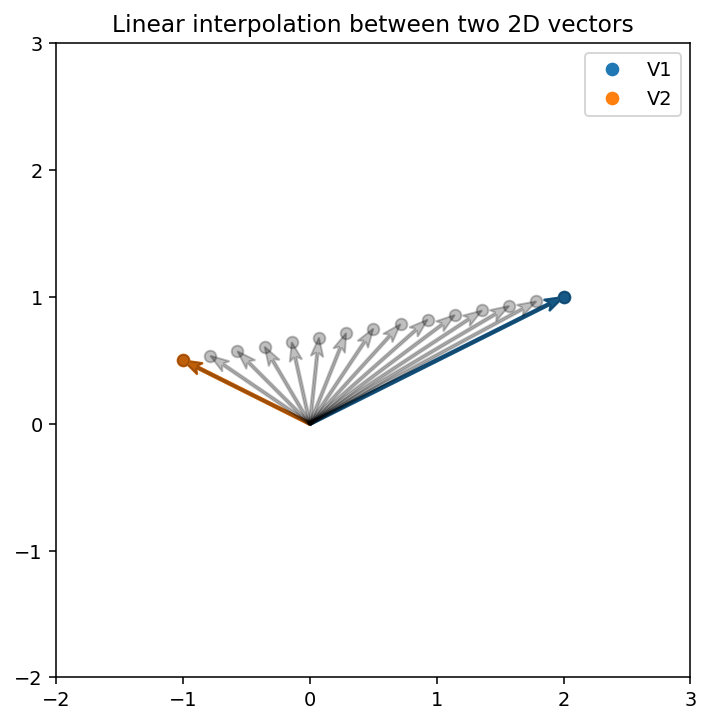
\includegraphics[scale=0.7]{src/3.1 lerp.png}
        \caption{An example of linear interpolation between two vectors.}
    \end{figure}

    \subsection{Norms}
    Not every vector space has a natural concept of distance, but $\mathbb{R}^n$ has a distance defined. The Euclidean length of a vector $\mathbf{x}$ is
    \[\lVert \mathbf{x} \rVert_2 = \sqrt{x_0^2 + x_1^2 + \dots + x_n^2}.\]
    It corresponds to the radius of the (hyper) sphere that would just touch the position specified by the vector. There are different norms in $\mathbb{R}^n$. For example, the $L_p$/Minkowski norms are given by
    \[\lVert \mathbf{x} \rVert_p = \sqrt[p]{x_0^p + x_1^p + \dots + x_n^p} = \sqrt[p]{\sum_{i=1}^{n} x_i^p}.\]
    Some common norms are:
    \begin{itemize}
        \item The $l_2$ norm (or the Euclidean norm) is the normal distance. Geometrically, the length corresponds to the radius of a sphere centered at the origin just touching the point;
        \item The $l_1$ norm (or the taxicab norm) gives the sum of absolute values. It is used to measure distances in high dimensions, or on grids. Geometrically, the length corresponds to the axis-aligned steps to get to that point;
        % \item The $l_0$ pseudo-norm just counts the number of non-zero elements;
        \item The $l_\infty$ norm gives the maximum element in the vector. It is used to capture maximum activation or excusion. Geometrically, the length corresponds to the length of a cube centered at the origin just touching this point;
        % \item The $l_{-\infty}$ norm gives the minimum element in the vector. It is used to capture minimum excusion.
    \end{itemize}
    
    A unit vector has norm 1. We can normalise a vector $\mathbf{x}$ by scaling it by $\frac{1}{\lVert \mathbf{x} \rVert}$. We typically talk about a unit vector with respect to the Euclidean norm. The Euclidean normalisation of random vectors in $\mathbb{R}^2$ is given below.
    \begin{figure}[H]
        \centering
        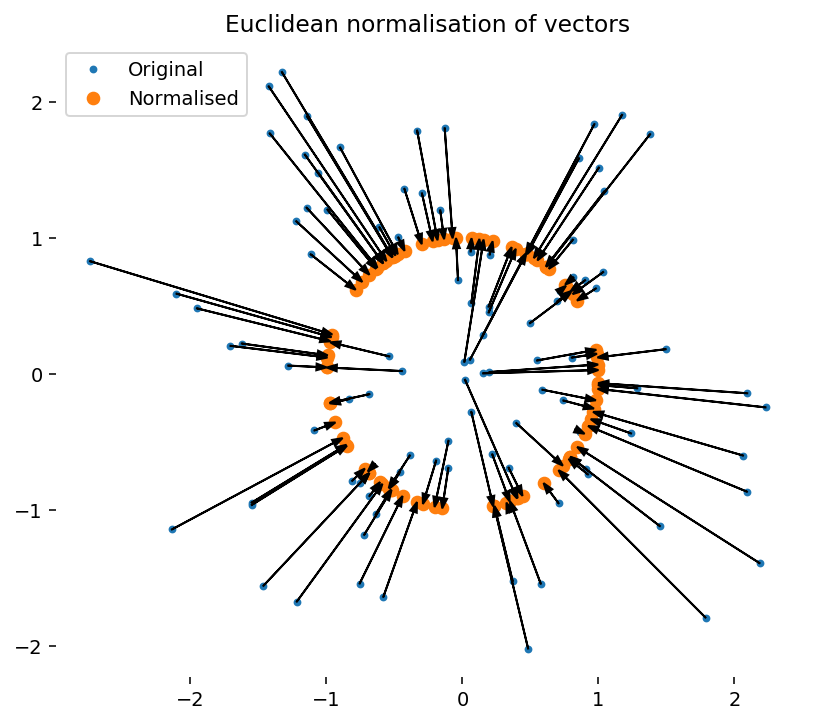
\includegraphics[scale=0.5]{src/3.2 Euclidean Normalisation.png}
        \caption{The Euclidean normalisation of random vectors in $\mathbb{R}^2$.}
    \end{figure}
    \noindent The $L_\infty$-normalisation of random vectors in $\mathbb{R}^2$ is given below.
    \begin{figure}[H]
        \centering
        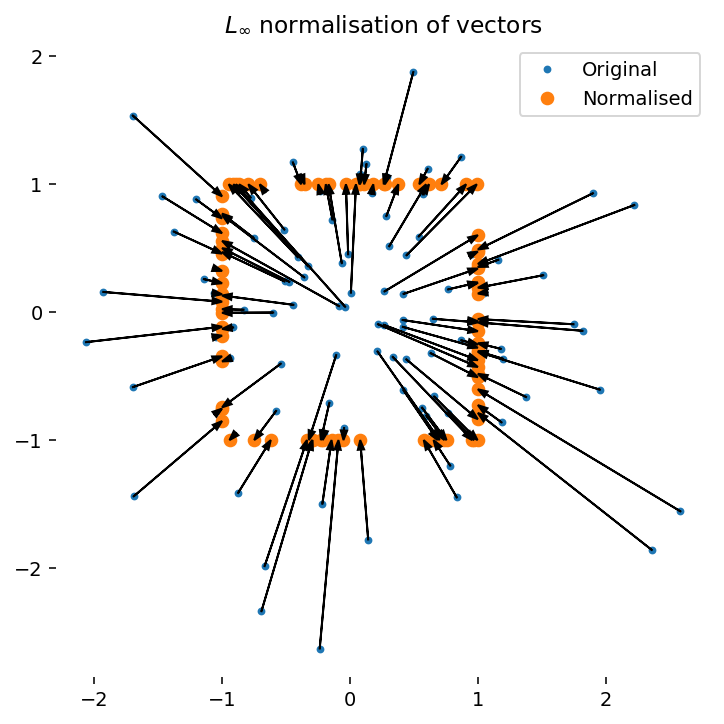
\includegraphics[scale=0.5]{src/3.3 Linfty Normalisation.png}
        \caption{The $L_\infty$-normalisation of random vectors in $\mathbb{R}^2$.}
    \end{figure}
    
    \subsection{Inner product}
    An inner product $(\mathbb{R}^n, \mathbb{R}^n) \to \mathbb{R}$ measures the angle between two real vectors. It is related to the cosine function:
    \[\cos (\theta) = \frac{\mathbf{x} \cdot \mathbf{y}}{\lVert \mathbf{x} \rVert \lVert \mathbf{y} \rVert}.\]
    The dot product of two vectors in $\mathbb{R}^n$ is given by
    \[\mathbf{x} \cdot \mathbf{y} = \sum_{i=0}^n x_i y_i.\]
    It is the sum of the elementwise products. Note that the vectors must have the same number of dimensions to perform this operation.

    We can use the inner product to compare vectors of different magnitudes- it does not depend on their magnitude, just their direction. For example, it is widely used in information retrieval to compare document vectors which represent terms present in a document as large, sparse vectors which might have wildly different magnitudes for documents of different lengths.

    \subsection{Mean Vector}
    The mean vector is the generalisation of the mean scalar, i.e.
    \[\sum_{i=1}^N \frac{1}{N} \mathbf{x}_i.\]
    The mean represents the geometric centroid of the vectors, and captures the center of mass of the vectors. By subtracting the mean from the dataset, we can center it with zero mean.
    \begin{figure}[H]
        \centering
        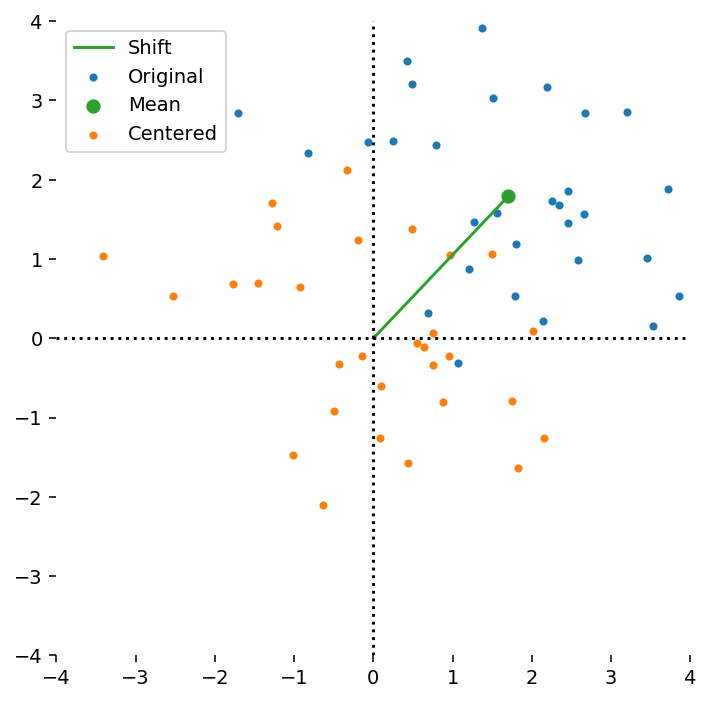
\includegraphics[scale=0.55]{src/3.4 Centered Data.png}
        \caption{Centering a dataset by subtracting the mean}
    \end{figure}

    There is no simple, direct algorithm to compute the median in higher dimensions. This is because the operation cannot be decomposed into scalar multiplication and addition.

    \section{Vectors in higher dimensions}
    Data science typically involves vectors with a lot of dimensions. For instance, a 512x512 image lives in $\mathbb{R}^{262 144}$. We can consider one data point to be a vector of measurements. Our choice of the measurements will impact the performance, behaviour of the algorithms.

    Geometry in higher dimensions is counter-intuitive. This is because the volume of space increases exponentially as the dimension increases. This means that there is a lot of empty space in higher dimensions. In particular, if data is sparse, it can be difficult to generalise in high-dimensional spaces.

    Many algorithms that work well with few dimensions do not genralise to higher dimensions. This is due to the curse of dimensionality.

    Consider the following histogram that represent data about temperature and humidity.
    \begin{figure}[H]
        \centering
        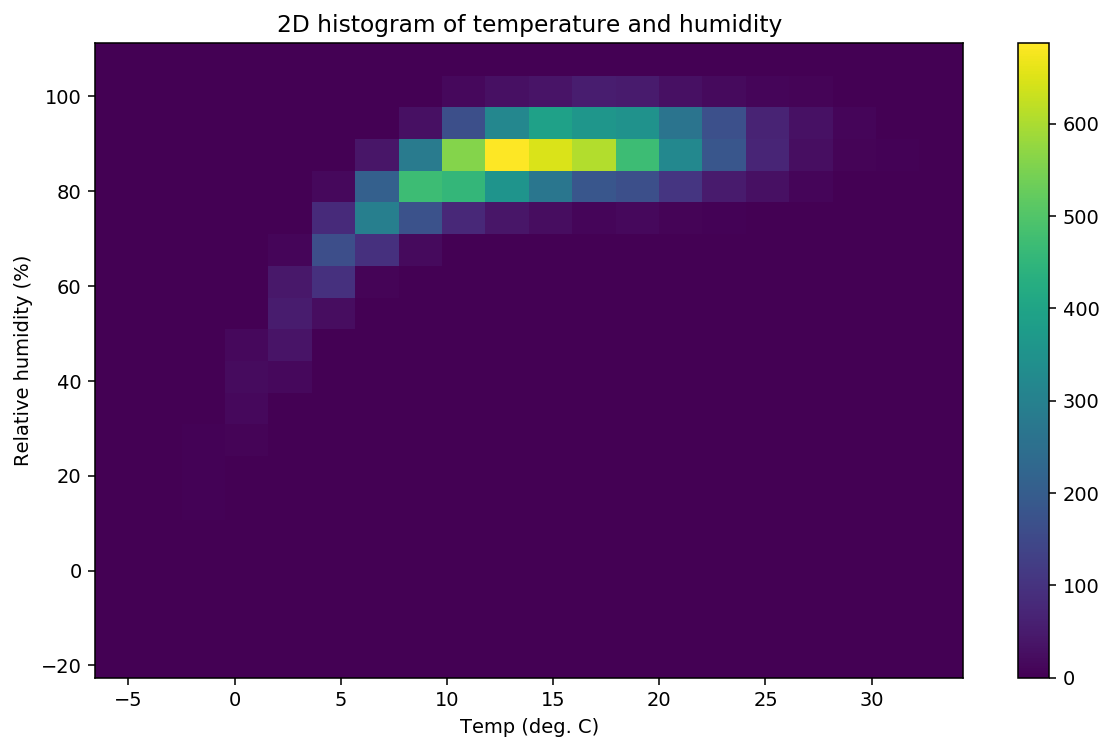
\includegraphics[scale=0.5]{src/3.5 2DHistogram.png}
        \caption{A 2D histogram}
    \end{figure}
    \noindent In the histogram above, there are 20 bins in each dimensions, for 400 bins total. Each bin only gets about 500 measurements, and in practice, most bins are empty and a few are heavily populatd. We cannot use histograms in higher dimensions because of the curse of dimensionality.

    If we had 10 different measurements (air temperature, air humidity, latitude, longitude, wind speed, wind direction, precipitation, time of day, solar power, sea temperature) and we wanted to subdivide them into 20 bins each, we would need a histogram with $20^{10}$ bins- over 10 trillion bins. This is the curse of dimensionality- as dimension increases, the generalisation gets harder exponentially.

    \subsection{Paradoxes in higher dimensions}
    We will try to find the volume of a (hyper)sphere within a cube as the dimension changes.
    \begin{figure}[H]
        \centering
        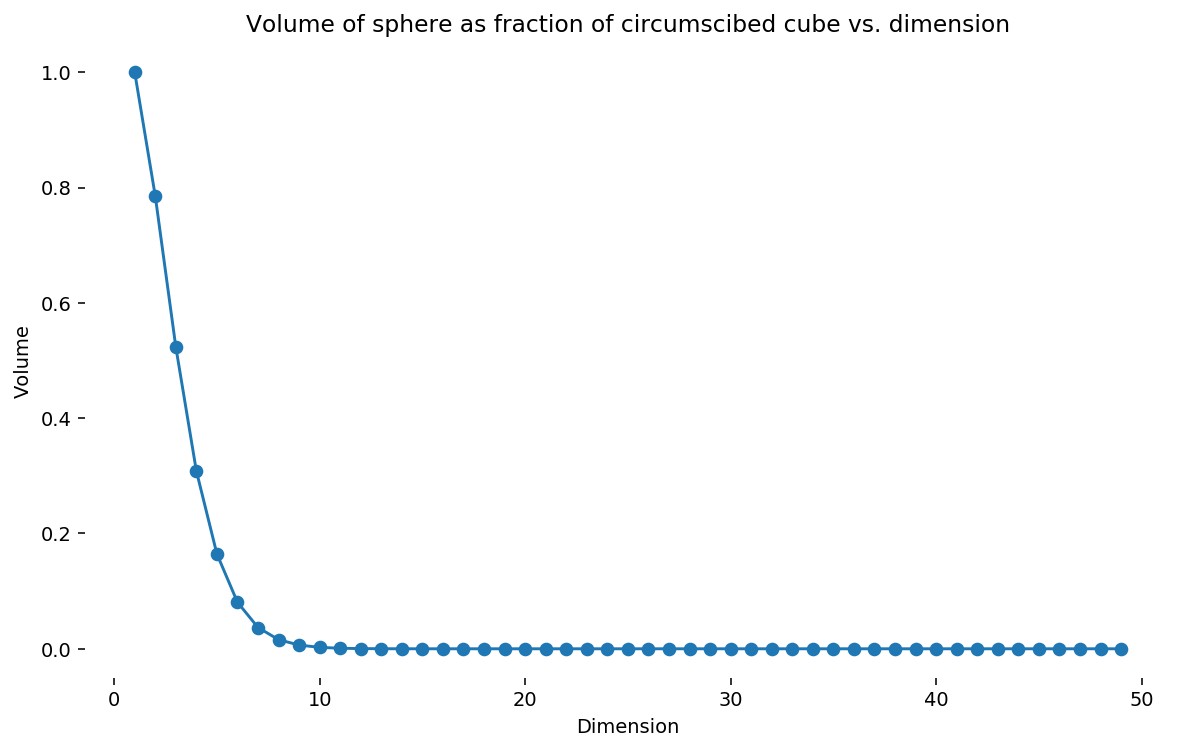
\includegraphics[scale=0.45]{src/3.6 VolumeVDimension.png}
        \caption{The volume of a sphere in a cube for various dimensions.}
    \end{figure}
    \noindent So, as the dimension increases, the volume of the sphere decreases; most of the values are in the corners.

    Moreover, if we randomly place points within the cube of high dimension, then most of the points are going to be outside of the cube. Furthemore, if we draw a line between two points on a hypercube, the points on the line still end up on the edge of the space. So, the distance between any two points using the Euclidean norm will almost always be the same. The figure below shows this.
    \begin{figure}[H]
        \centering
        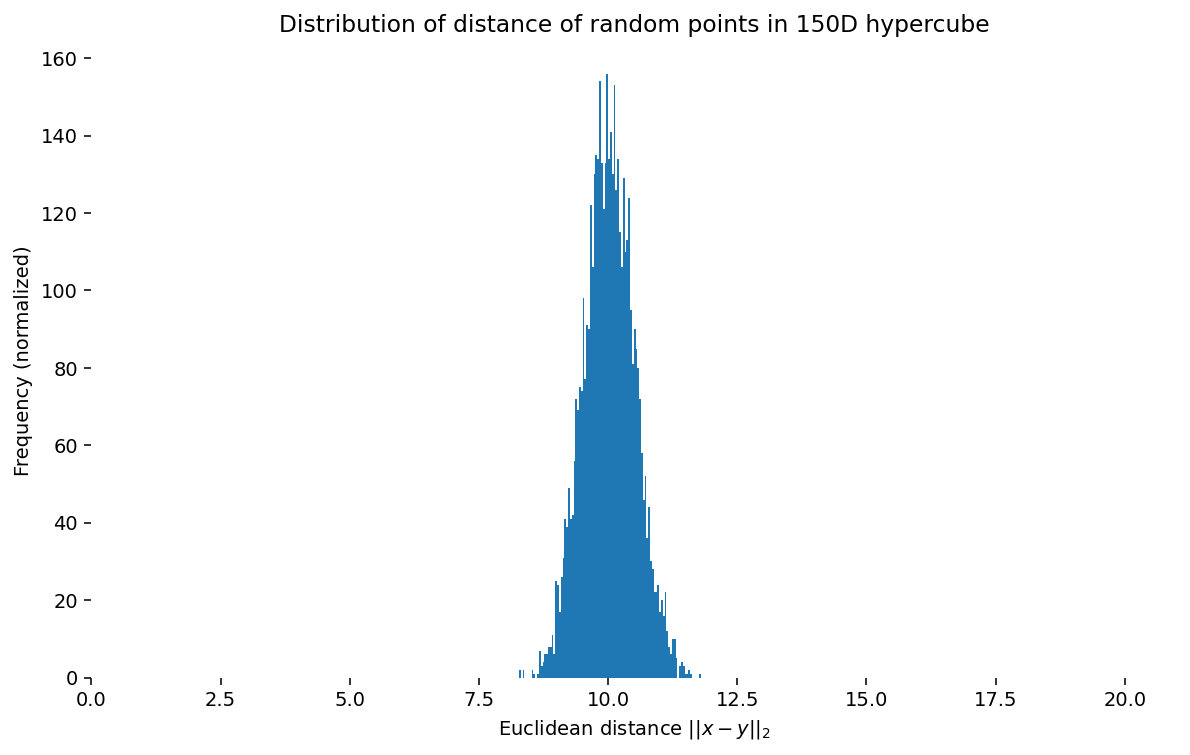
\includegraphics[scale=0.45]{src/3.8 Distribution of distance of random points 150D.png}
        \caption{Distribution of distance of random points in a 150D hypercube, with respect to the Euclidean norm.}
    \end{figure}
    If we instead look at the 2D case, we get an expected result.
    \begin{figure}[H]
        \centering
        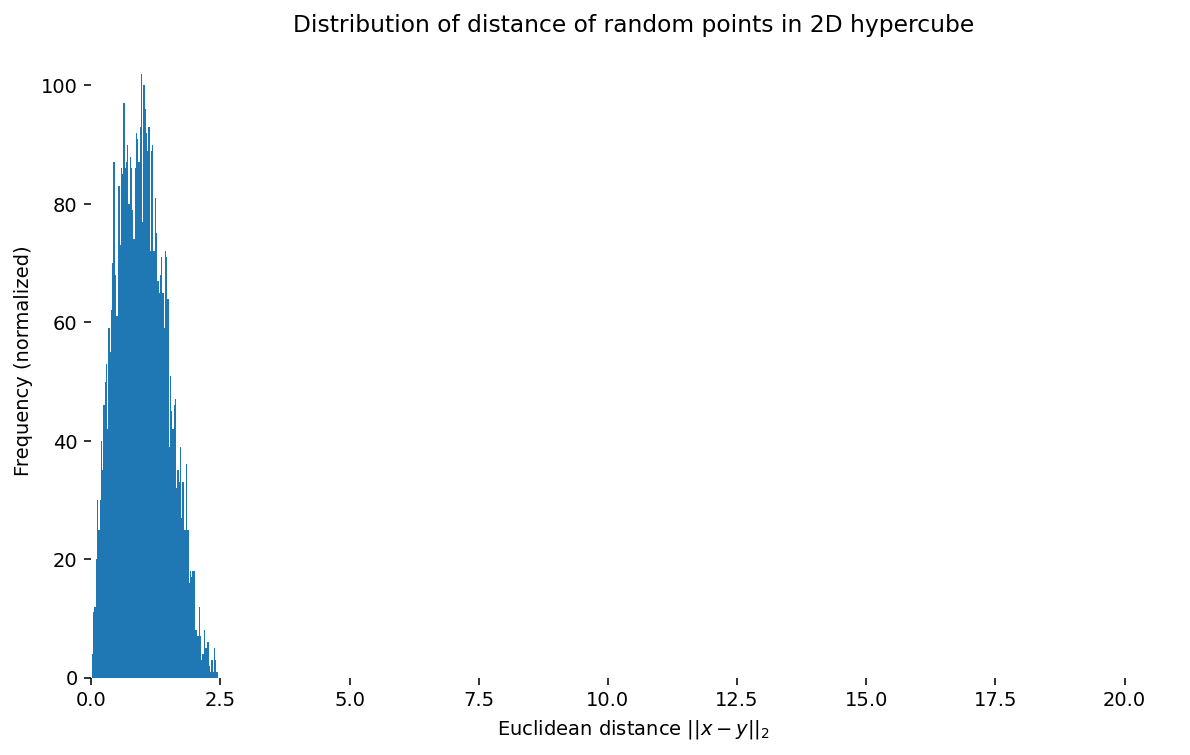
\includegraphics[scale=0.45]{src/3.9 Distribution of distance of random points 2D.png}
        \caption{Distribution of distance of random points in a 2D hypercube, with respect to the Euclidean norm.}
    \end{figure}
    \noindent We expect the distance between any two points to be spread- between some vectors, the distance could be quite close to 0. However, this just isn't true in higher dimensions, as we can see above. Other norms (e.g. $L_1$ and $L_\infty$) are less sensitive to the curse, but they aren't perfect.

    \section{Matrices}
    Matrices are 2D arrays of reals: $\mathbb{R}^{n \times m}$ ($n$ rows and $m$ columns). Vectors represent point in space; matrices represent operations to transform vectors. Operations defined by matrices are rigid transformations.
    \subsection{Matrix operations}
    Matrices can be:
    \begin{itemize}
        \item added/subtracted- $(\mathbb{R}^{n \times m}, \mathbb{R}^{n \times m})\to \mathbb{R}^{n \times m}$;
        \item scaled (by a scalar)- $(\mathbb{R}^{n \times m}, \mathbb{R}) \to \mathbb{R}^{n \times m}$;
        \item transposed (rows and columns flipped)- $\mathbb{R}^{n \times m} \to \mathbb{R}^{m \times n}$;
        \item applied to vectors- $(\mathbb{R}^{n \times m}, \mathbb{R}^m) \to \mathbb{R}^n$;
        \item multiplied (i.e. which composes the transformations)- $(\mathbb{R}^{p \times q}, \mathbb{R}^{q \times r}) \to \mathbb{R}^{p \times r}$.
    \end{itemize}

    Matrices represent linear maps of vectors. That is, a matrix is like a function that can be applied to a vector by multiplication, i.e. $f(\mathbf{x}) = A \mathbf{x}$. A matrix representation presents the function in a very compact way.

    If we have an $n \times m$ matrix, then the matrix $A$ represents a function $(\mathbb{R}^m) \to \mathbb{R}^n$ such that
    \begin{itemize}
        \item all straight lines remain straight;
        \item all parallel lines remain parallel; and
        \item the origin does not move.
    \end{itemize}
    This is equivalent to saying that:
    \begin{align*}
        f(\mathbf{x}+\mathbf{y}) = f(\mathbf{x}) + f(\mathbf{y}) &= A(\mathbf{x}+\mathbf{y}) = A(\mathbf{x}) + A(\mathbf{y}) \\
        f(c\mathbf{x}) = cf(\mathbf{x}) &= A(c\mathbf{x}) = cA(\mathbf{x}).
    \end{align*}
    This property is linearity, and matrices represent linear maps.

    A linear map is a function $f: \mathbb{R}^m \to \mathbb{R}^n$ that satisfy the linearity conditions. An $n \times n$ matrix matrix maps from the vector space to itself $(\mathbb{R}^n) \to \mathbb{R}^n$- this is called a linear transform. If a map satisfies $AAx = Ax$, i.e. $f(f(x)) = f(x)$, then it is called a linear projection, e.g. it projects 3D points into a 2D plane. Every linear map of real vectors can be written as a real matrix.

    We will now look at some examples of matrix transformations in 2D:
    \begin{itemize}
        \item The identity transformation is given by the matrix $\begin{bmatrix}
            1 & 0 \\
            0 & 1
        \end{bmatrix}$. The following is its transformation.
        \begin{figure}[H]
            \centering
            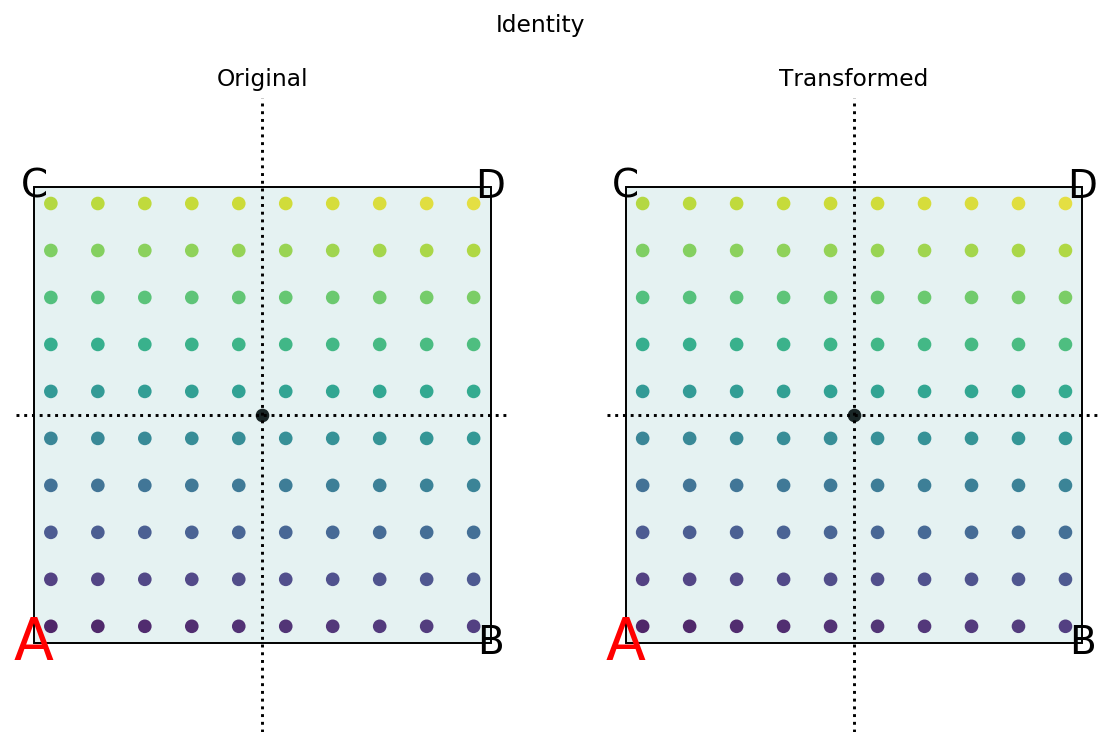
\includegraphics[scale=0.5]{src/3.10 IdentityTransformation.png}
            \caption{The identity transformation to the 2D plane.}
        \end{figure}    
        
        \item The matrix given by $\begin{bmatrix}
            0.5 & 0 \\
            0 & 0.5
        \end{bmatrix}$ uniformly scales the plane. The following is its transformation.
        \begin{figure}[H]
            \centering
            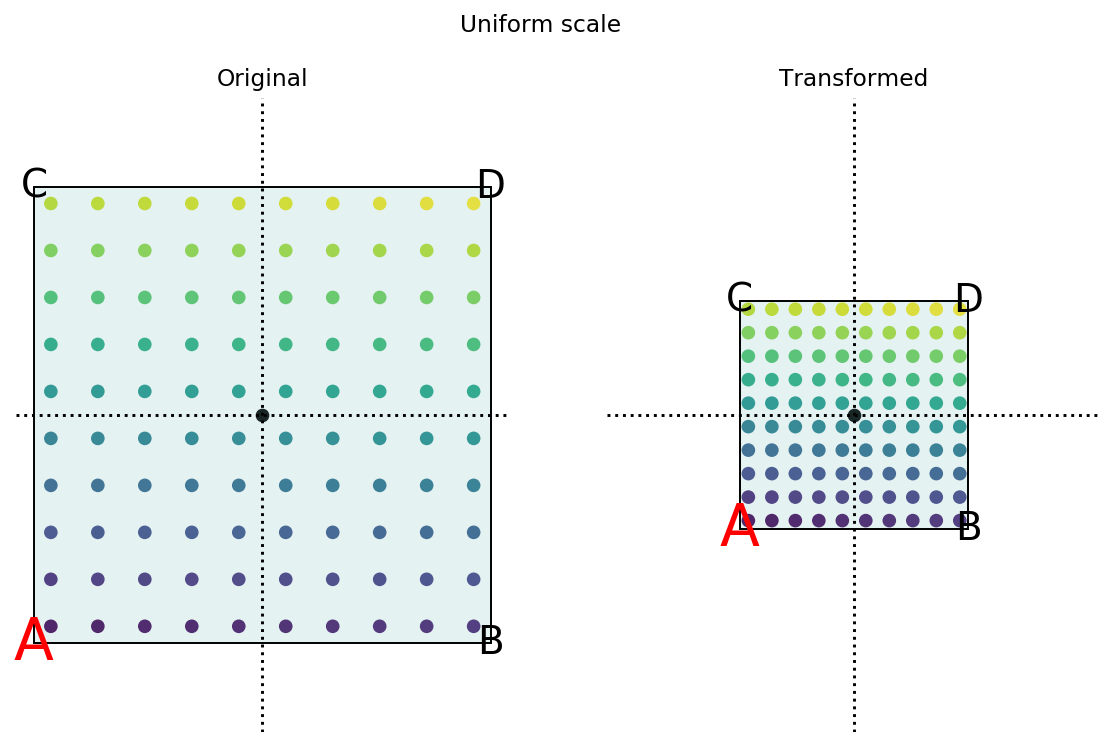
\includegraphics[scale=0.5]{src/3.11 UniformScale.png}
            \caption{A uniform scaling transformation to the 2D plane.}
        \end{figure}    

        \item The matrix given by $\begin{bmatrix}
            0.5 & 0 \\
            0 & 1
        \end{bmatrix}$ scales the plane in a non-uniform manner (only the $x$-axis). The following is its transformation.
        \begin{figure}[H]
            \centering
            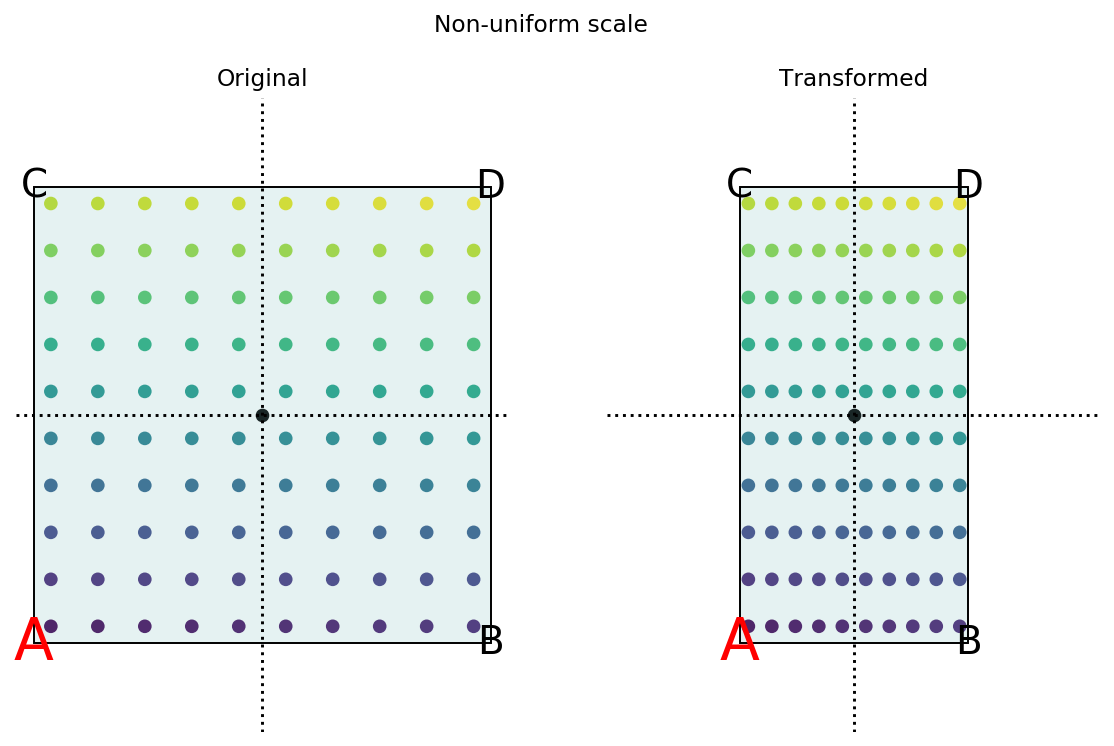
\includegraphics[scale=0.5]{src/3.12 NonUniformScale.png}
            \caption{A non-uniform scaling transformation to the 2D plane.}
        \end{figure}    

        \item The matrix given by $\begin{bmatrix}
            0 & 1 \\
            -1 & 0
        \end{bmatrix}$ rotates the plane by $90^{\circ}$. The following is its transformation.
        \begin{figure}[H]
            \centering
            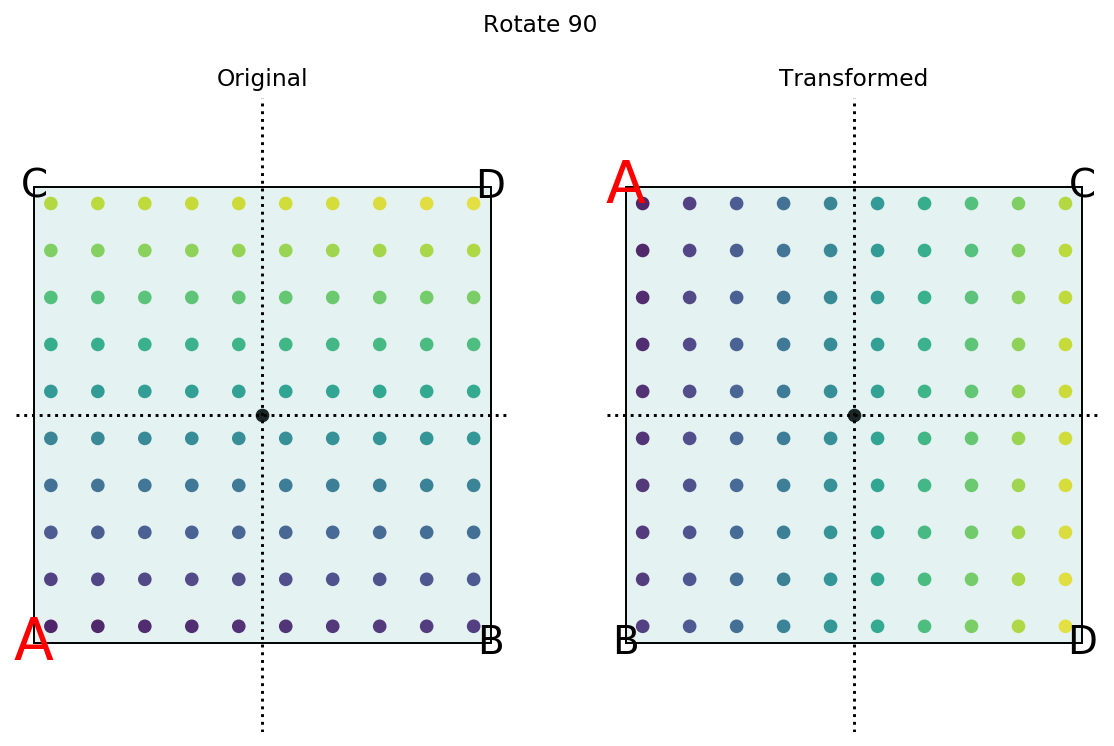
\includegraphics[scale=0.5]{src/3.13 Rot90.png}
            \caption{A rotation transformation to the 2D plane.}
        \end{figure}    

        \item The matrix given by $\begin{bmatrix}
            -1 & 0 \\
            0 & 1
        \end{bmatrix}$ flips the $x$-axis. The following is its transformation.
        \begin{figure}[H]
            \centering
            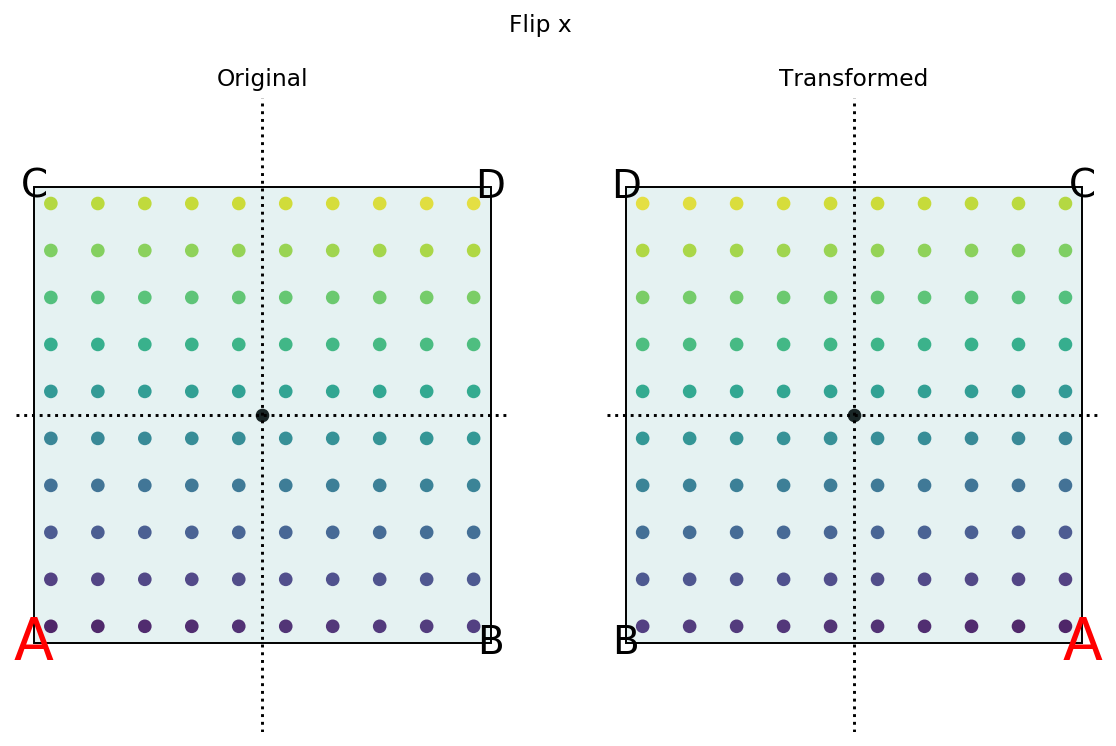
\includegraphics[scale=0.5]{src/3.14 FlipX.png}
            \caption{The transformation to the 2D plane which flips the $x$-axis.}
        \end{figure}    

        \item The matrix given by $\begin{bmatrix}
            0.15 & 0.75 \\
            0.5 & 0.8
        \end{bmatrix}$ has a shearing effect to the plane. The following is its transformation.
        \begin{figure}[H]
            \centering
            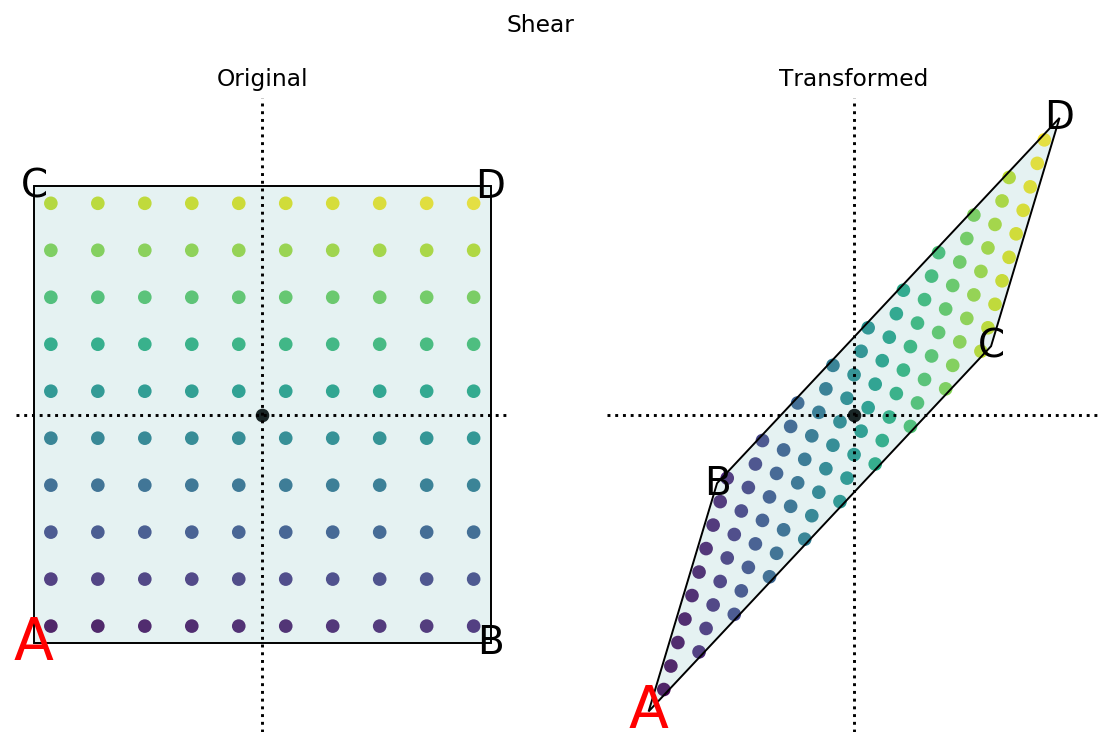
\includegraphics[scale=0.4]{src/3.15 Shear.png}
            \caption{A shear transformation to the 2D plane.}
        \end{figure}    
    \end{itemize}

    We can apply a matrix to a vector. An application takes a weighted sum of the elements (linear combinations) within a vector. If we have an $n \times m$ matrix, then it is a function that maps from an $m$-dimensional vector space to an $n$-dimensional vector space.

    We can also multiply matrices. Multiplication composes the effect of the two matrices, i.e. $BA = g(f(x))$, where $g(x)= Bx$ and $f(x) = Ax$. The product $AB$ only makes sense if $A$ is $p \times q$ and $B$ is $q \times r$- $AB$ will be $p \times r$. The product $AB$ is $B$ left-multiply $A$, and $A$ right-multiply $B$.

    Matrix multiplication has complexity $O(pqr)$. If the matrices are square, then it is $O(n^3)$. There are special forms of matrices which can be multiplied much faster. There are optimised/accelerated algorithms, but they are always worse than $O(n^2)$. Most accelerated algorithms are impractical for all but the largest matrices because they have enormous constant overhead.

    We illustrate matrix multiplication by combining two transformations: the matrix that rotates the 2D plane by $30^{\circ}$ and the matrix that scales the $x$-axis by $1/2$, and leaves the $y$-axis. If we first rotate then scale, we get the following transformation.
    \begin{figure}[H]
        \centering
        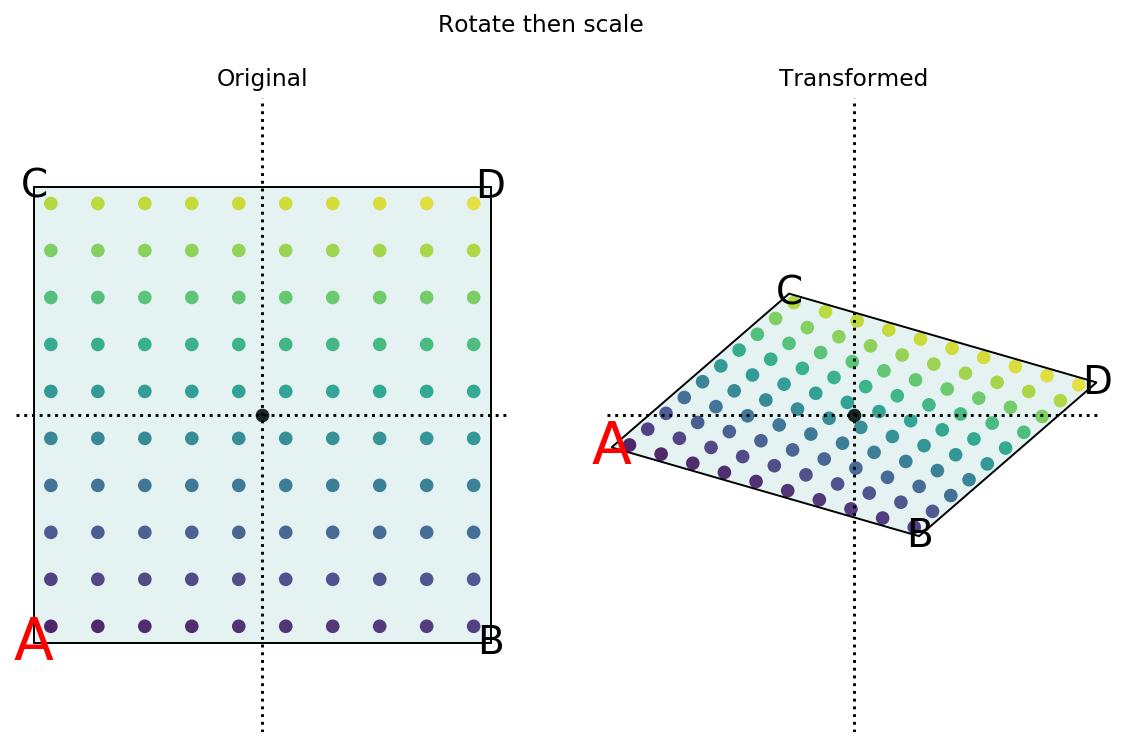
\includegraphics[scale=0.4]{src/3.18 RotateScale.png}
        \caption{A transformation composed of rotating then scaling.}
    \end{figure}    
    \noindent Instead, if we scale then rotate, we get the following transformation.
    \begin{figure}[H]
        \centering
        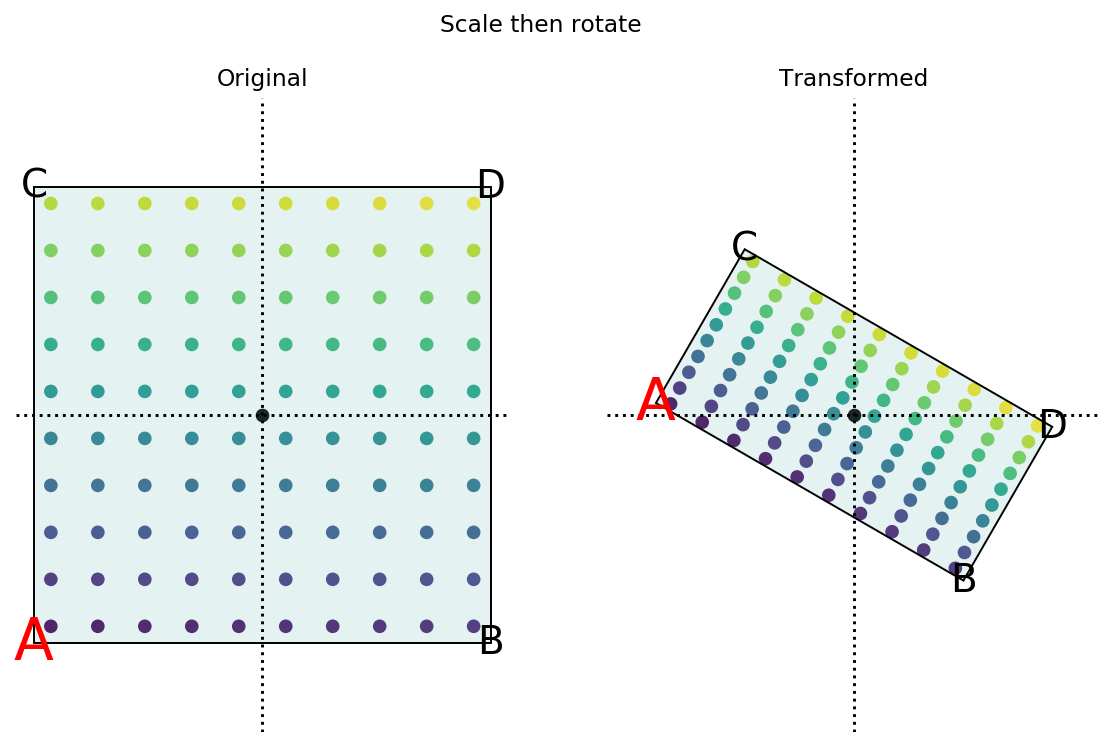
\includegraphics[scale=0.4]{src/3.19 ScaleRotate.png}
        \caption{A transformation composed of scaling then rotating.}
    \end{figure}

    As we can see above, composition of two matrices depends on the order, i.e. $AB \neq BA$. We say that matrix multiplication is not commutative. Moreover, just because the matrix $AB$ is defined doesn't mean that the matrix $BA$ is defined. In fact, for both $AB$ and $BA$ to be defined, the two matrices need to both be $n \times n$.

    Applying a vector to a matrix is like multiplying an $n \times m$ matrix with an $m \times 1$ matrix (i.e. a column vector), and produces an $n \times 1$ matrix.

    We can transpose a matrix- this flips the rows and the columns. For instance,
    \[\begin{bmatrix}
        2 & -5 \\
        1 & 0 \\
        3 & 3
    \end{bmatrix}^T = \begin{bmatrix}
        2 & 1 & 3 \\
        -5 & 0 & 3
    \end{bmatrix}.\]
    We only change the strides in the header, so this operation takes constant time. In 1D, the transpose of a row vector is a column vector. We can define the inner product of two vectors using matrix multiplication and transpose, i.e. $\mathbf{x} \cdot \mathbf{y} = \mathbf{x}\mathbf{y}^T$. This gives rise to the outer product $\mathbf{x} \otimes \mathbf{y} = \mathbf{x}^T \mathbf{y}$. The result is an $n \times n$ matrix.

    The transposition of a product is given by $(AB)^T = B^T A^T$. If $A$ is $p \times q$ and $B$ is $q \times r$, then $B^T$ is $r \times q$ and $A^T$ is $q \times r$. Also, $(A + B)^T = A^T + B^T$.

    \section{Covariance Matrix}
    Along with the mean vector, we can compute the variation/spread found in the dataset. In the 1D case, variance is given by
    \[\frac{1}{N-1} \sum_{i=0}^{N-1} (x_i - \mu)^2.\]
    It measures how spread out the values $x_i$ are, to the mean. The standard deviation is the square root of the variance- it has the same units as $\mathbf{x}$.

    In the multi-dimensional case (i.e. $N \times d$ data matrix $X$, with $N$ $d$-dimensional vectors), we compute the covariance of every dimension with every other dimension. This is the average squared distanceof every column of data from the average of every column. So, the entry $(i, j)$ is given by
    \[\frac{1}{N-1} \sum_{i=0}^{N-1} (X_{ki} - \mu_i) (X_{kj} - \mu_j).\]
    We can visualise the covariance matrix by an ellipse. This represents an (inverse) transform of a unit sphere to an ellipse covering the data. The mean vector is the center of the ellipse. The ellipse is sometimes called the error ellipse.
    \begin{figure}[H]
        \centering
        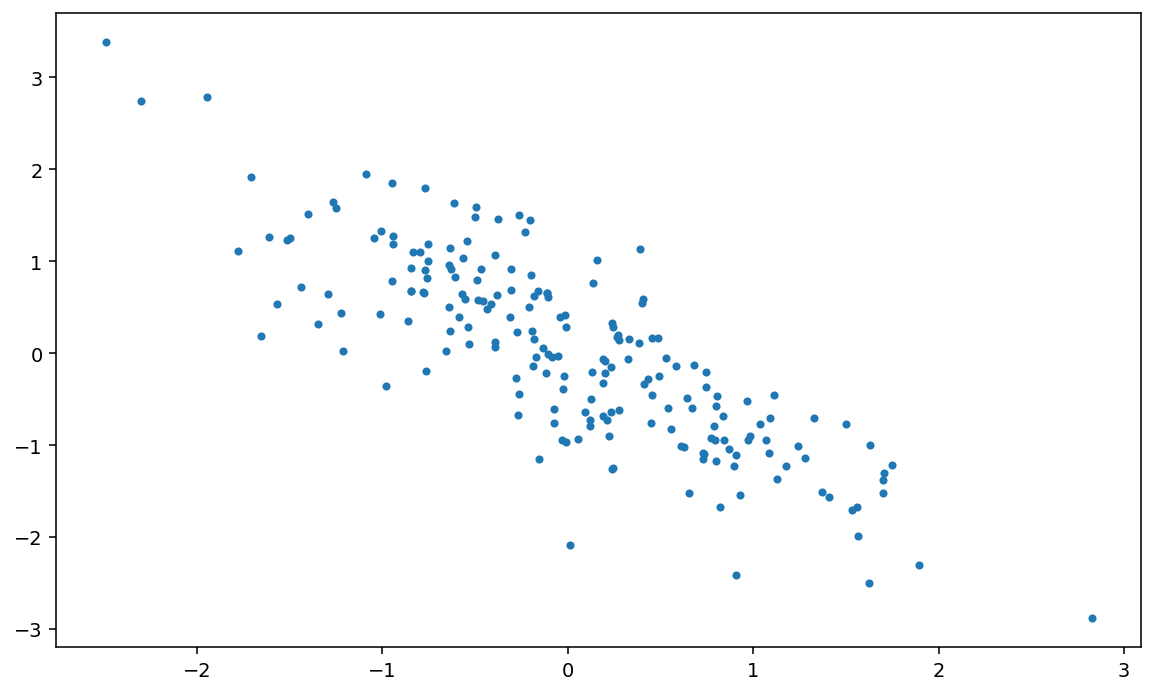
\includegraphics[scale=0.5]{src/3.20 covariance ellipse.png}
        \caption{The covariance ellipse.}
    \end{figure}

    The covariance matrix and the mean vector generalise the concepts of standard deviation and the mean scalar in the real case respectively. In particular, the mean vector represents the center of the data points, and the covariance matrix the spread of the data.

    \section{Types of matrices}
    We now look at different types of matrices:
    \begin{itemize}
        \item An $n \times n$ matrix with only non-zero entries in the main diagonal is called a diagonal matrix. These matrices represent the transformation that scales each dimension of the vector separately. All angles remain unchanged- there is no rotation performed. For example, the matrix 
        \[\begin{bmatrix}
            1 & 0 & 0 \\
            0 & 2 & 0 \\
            0 & 0 & 3
        \end{bmatrix}\]
        is a diagonal matrix.

        \item An $n \times n$ matrix with only non-zero entries in the off diagonal is called an anti-diagonal matrix. For example, the matrix 
        \[\begin{bmatrix}
            0 & 0 & 1 \\
            0 & 1 & 0 \\
            1 & 0 & 0
        \end{bmatrix}\]
        is an anti-diagonal matrix.
    
        \item The identity matrix $I$ is the $n \times n$ matrix with zero entries in the non-diagonals and ones everywhere in the diagonal. The identity matrix has no effect on a vector/matrix. That is, $Ix = x = xI$ and $IA = A = AI$, given that the dimension of $I$ is compatible. For example, the $3 \times 3$ identity matrix is
        \[\begin{bmatrix}
            1 & 0 & 0 \\
            0 & 1 & 0 \\
            0 & 0 & 1
        \end{bmatrix}.\]
    
        \item A scalar multiple of the identity matrix has the effect of uniformly scaling all the dimensions of a vector.
    
        \item The zero matrix $O$ is the $m \times n$ matrix with zero entries everywhere. Multiplying any vector/matrix with the zero matrix $O$ will give the zero vector/matrix- it maps everything to the origin.
    
        \item An $n \times n$ matrix is called a square matrix. These matrices transform a vector in $\mathbb{R}^n$ to another vector in $\mathbb{R}^n$. There are many properties only defined on square matrices.
    
        \item A square matrix is triangular if it has non-zero entries above (upper triangular) or non-zero entries below (lower triangular) the diagonal. For example, the matrix 
        \[\begin{bmatrix}
            1 & 0 & 0 \\
            1 & 2 & 0 \\
            1 & 1 & 3
        \end{bmatrix}\]
        is lower-triangular matrix, and the matrix 
        \[\begin{bmatrix}
            1 & 2 & 2 \\
            0 & 2 & 2 \\
            0 & 0 & 3
        \end{bmatrix}\]
        is an upper-triangular diagonal matrix. The corresponding system of equations can be very easily solved by substitution.
    
        \item A square matrix $A$ is symmetric if $A = A^T$. The covariance matrix is always symmetric. For example, the matrix 
        \[\begin{bmatrix}
            1 & 1 & 2 \\
            1 & 2 & 3 \\
            2 & 3 & 3
        \end{bmatrix}\]
        is a symmetric matrix.
    \end{itemize}

    \section{Graphs and matrices}
    We can represent (directed) graphs using (adjacency) matrices. For each pair of vertices in the graph, if they have an edge, the entry is 1, otherwise the entry is 0.

    A graph has the following properties:
    \begin{itemize}
        \item the in-degree of a vertex- the number of vertices which have an edge leading to this vertex. This is the sum of the column that the vertex represents.
        \item the out-degree of a vertex- the number of vertices which have an edge going from this vertex. This is the sum of the row that the vertex represent.
        \item if the matrix is symmetric, then it is undirected- we can make any matrix symmetric by adding its transpose. In the case of graphs, this makes the edges bi-directional.
        \item if there is a non-zero diagonal entry, then there is an edge going from the vertex to itself (self-transition).
    \end{itemize}

    It is possible to have weights associated with the edges. We can easily adapt our matrix representation to add this data- we make the entry in the matrix equal to the value of the weight.

    For instance, assume that we have a graph that shows the flow of packages from depots. Then,
    \begin{itemize}
        \item if the total flow out of a vertex is $> 1$ (i.e. its rows sum to $> 1$), then the vertex is a source- the depot produces some products;
        \item if the total flow out of a vertex is $< 1$, then it is a sink- the depot makes use of some products;
        \item if the total flow out of a vertex is exactly 1, then it conserves mass- it reroutes everything.
    \end{itemize}
    If the whole graph consists of vertices whose total outgoing weight is 1, and all weights are positive or zero, then the whole graph preserves mass under flow. Nothing is produced or consumed. Each row in the adjacency matrix sums to 1. This is called a conserving adjacency matrix. We can normalise the rows of any matrix (so long as each vertex has at least some flow out of it) to form a conserving adjacency matrix.

    \subsection{Flow analysis}
    We can use matrices to model discrete problems. For examples, matrices can be used to keep track of how many packages at each depot at an instant in time, and therefore predict how many packages will be there tomorrow/how many were there yesterday.

    In particular, we can find some matrix $A$ such that
    \[\mathbf{x}_1 = A \mathbf{x}_0,\]
    where $\mathbf{x}_0$ is the number of packages in each depot today (as a vector), and we want to predict $\mathbf{x}_1$- the number of packages in each depot tomorrow. The advantage of vectorised operations is that they can be accelerated using hardware such as a GPU (Graphical Process Unit).

    Using matrices, we can attempt to answer the following:
    \begin{itemize}
        \item What about in a week's time? What will $x_7$ be?
        \item What about in one hour's time (i.e. a 24th of a day)? What will be $x_{1/24}$ be?
        \item What about at time $x_{\infty}$? What is the long term behaviour? Will the system reach a steady state (an equilibrium)? Or will it oscillate forever?
        \item What about if we wanted to go backwards in time? If we know $x_0$, can we predict yesterday $x_{-1}$?
    \end{itemize}

    \section{More matrix operations}
    \subsection{Exponentiation}
    For a square matrix $A$, we can apply the square to itself, i.e. $A^k = AA \dots A$. This allows us to compute the value in a week's time- this is $A^7 \mathbf{x}_0$.

    We illustrate how a rotation matrix $A$ can be exponentiated in 2D.
    \begin{itemize}
        \item The matrix $A^0$ is the identity transformation.
        \begin{figure}[H]
            \centering
            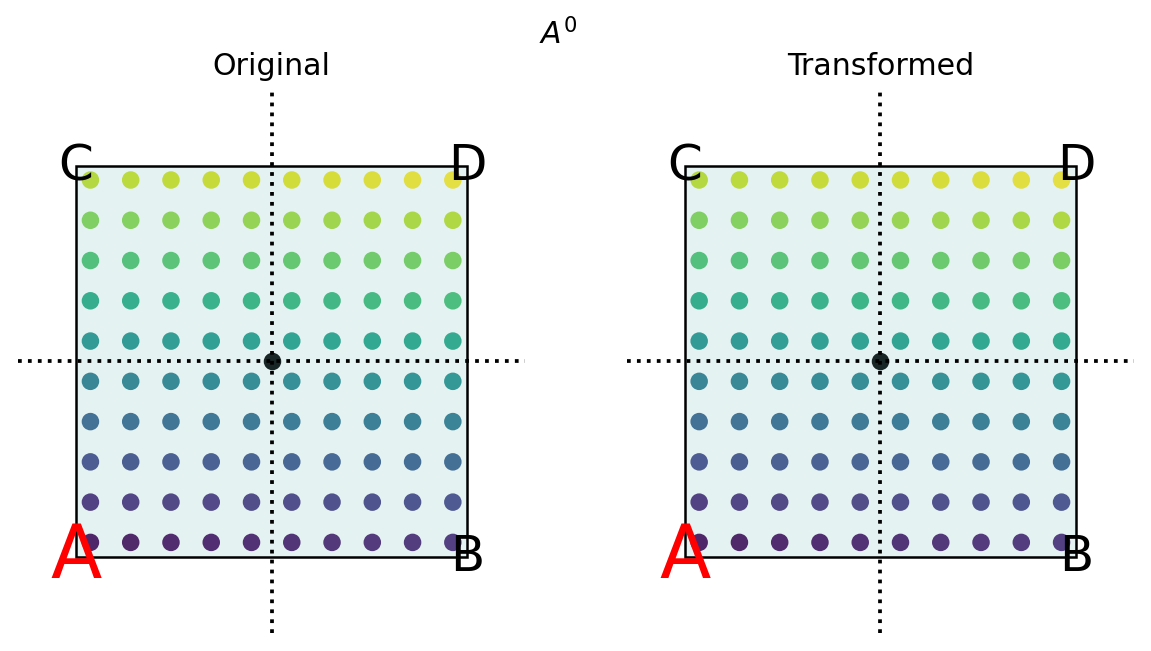
\includegraphics[scale=0.4]{src/3.21 A^0.png}
            \caption{The 2D plane transformation by $A^0$.}
        \end{figure}

        \item The matrix $A$ is a rotation transformation.
        \begin{figure}[H]
            \centering
            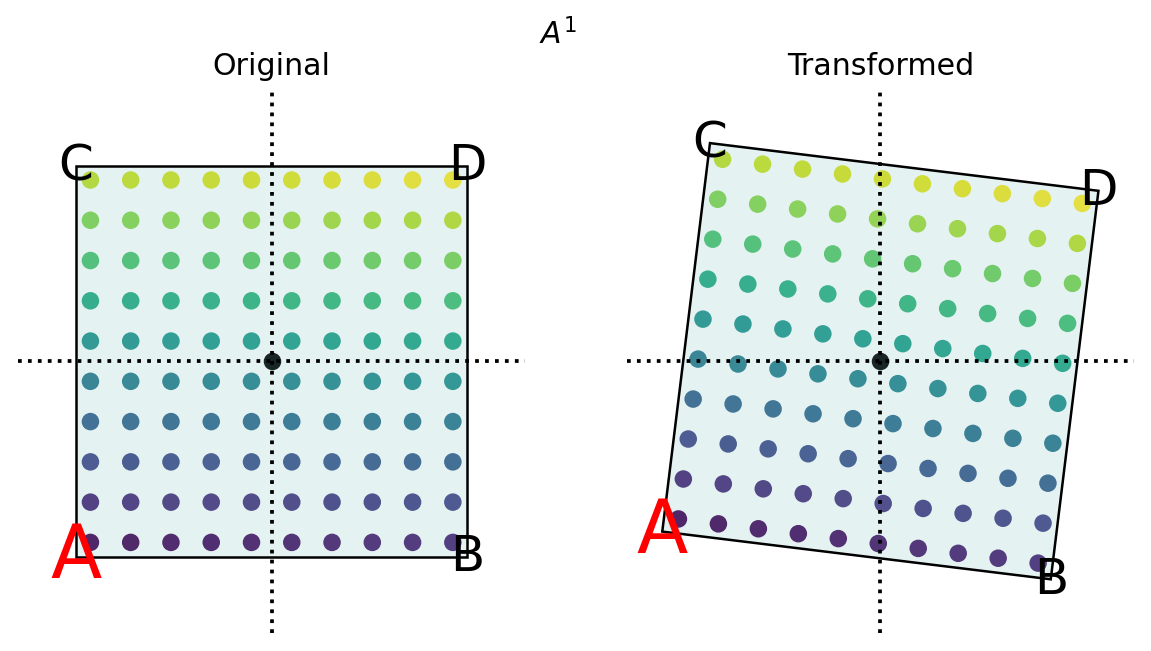
\includegraphics[scale=0.4]{src/3.22 A^1.png}
            \caption{The 2D plane transformation by $A$.}
        \end{figure}
        
        \item The matrix $A^2$ is rotates the 2D plane by double the degree of the rotation by $A$.
        \begin{figure}[H]
            \centering
            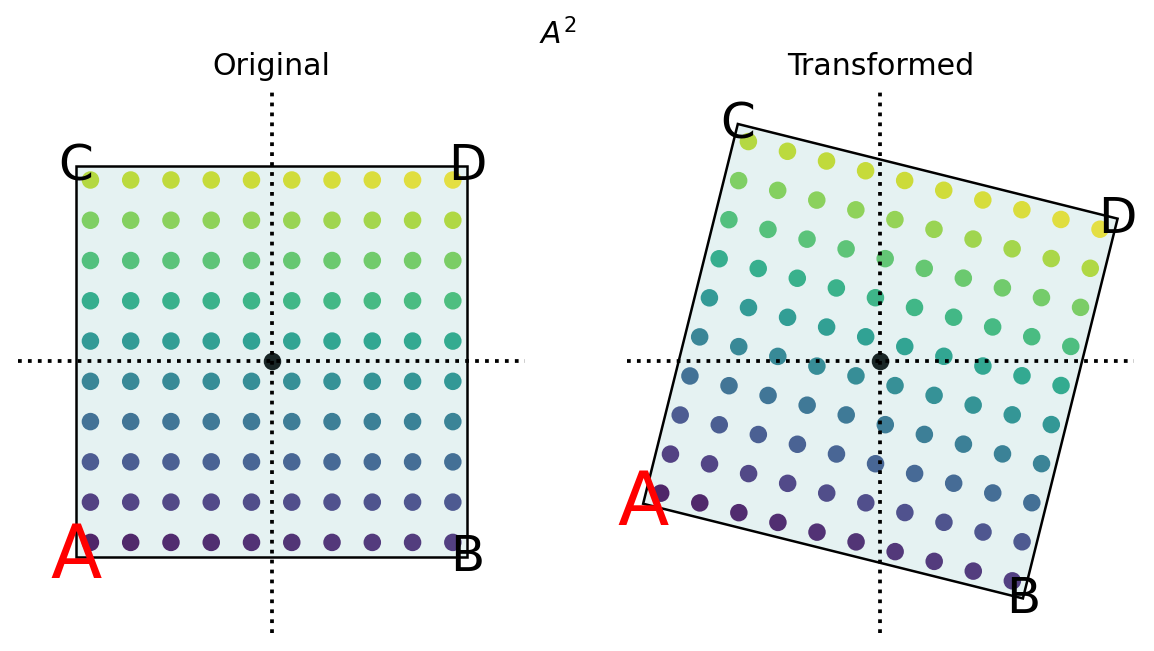
\includegraphics[scale=0.4]{src/3.23 A^2.png}
            \caption{The 2D plane transformation by $A^2$.}
        \end{figure}
    \end{itemize}
    
    \section{Eigenvalues and eigenvectors}
    Consider the depot example again. We can see how the packages flow over time, where we vary the initial depot.
    \begin{figure}[H]
        \centering
        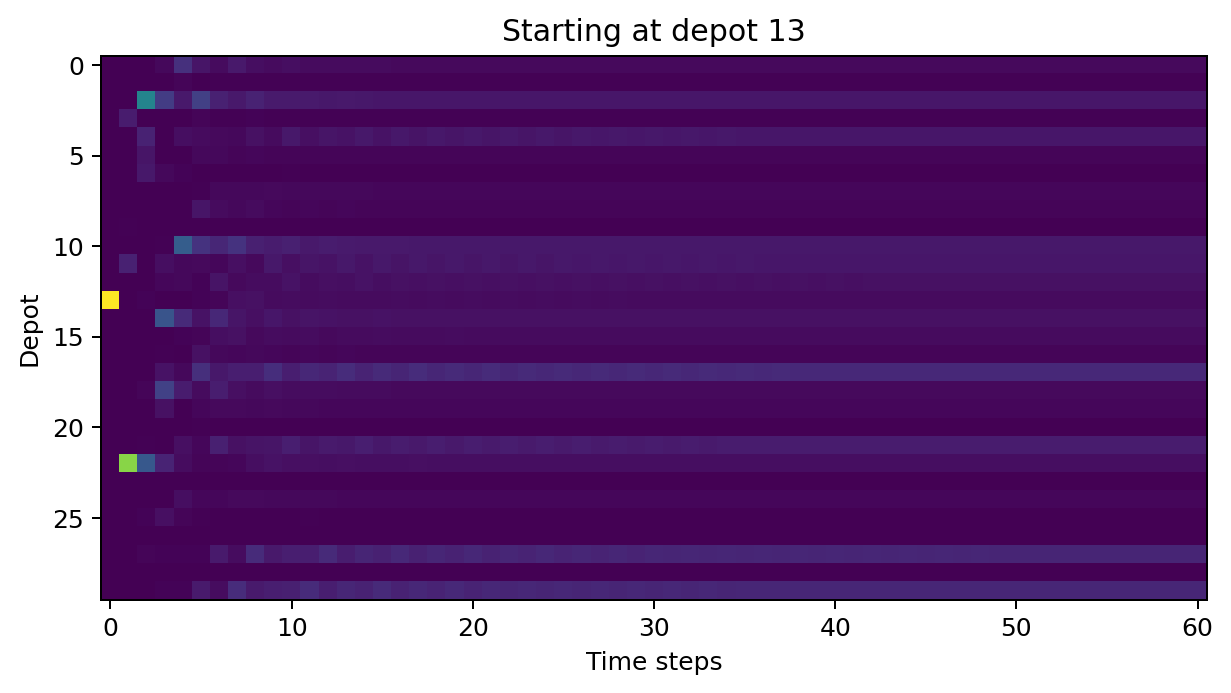
\includegraphics[scale=0.4]{src/3.24 Start at 13.png}
        \caption{The evolution of package locations over time, starting at depot 13.}
    \end{figure}
    \begin{figure}[H]
        \centering
        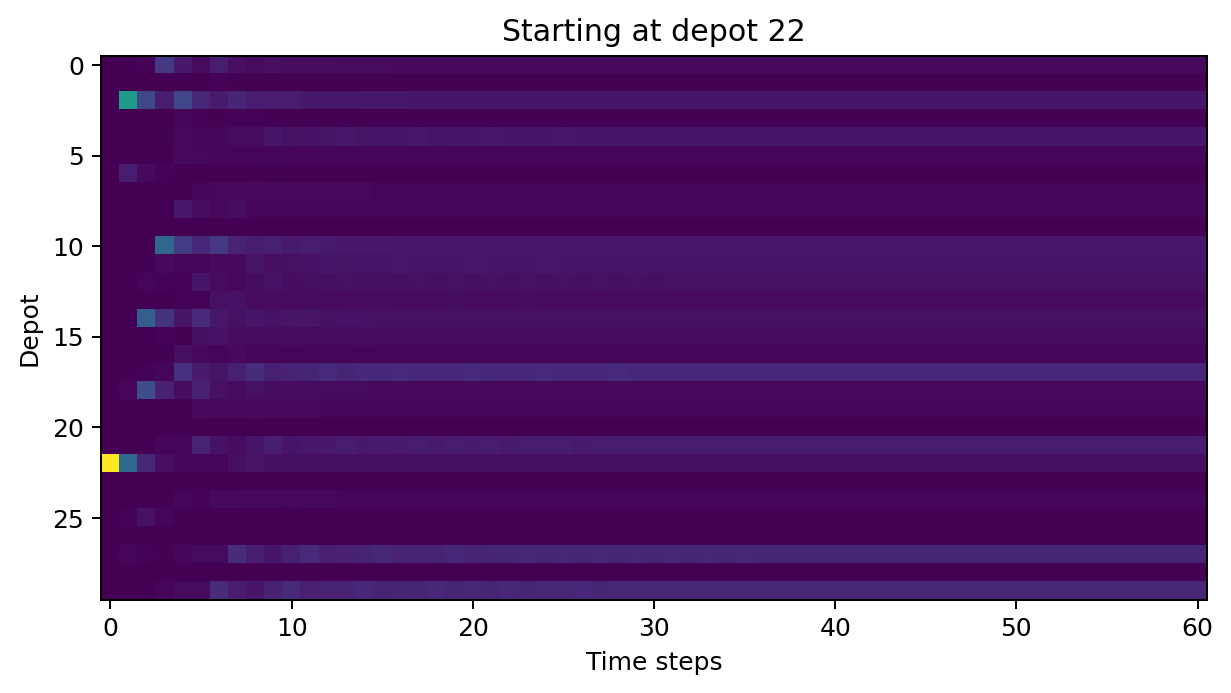
\includegraphics[scale=0.4]{src/3.25 Start at 22.png}
        \caption{The evolution of package locations over time, starting at depot 22.}
    \end{figure}
    \begin{figure}[H]
        \centering
        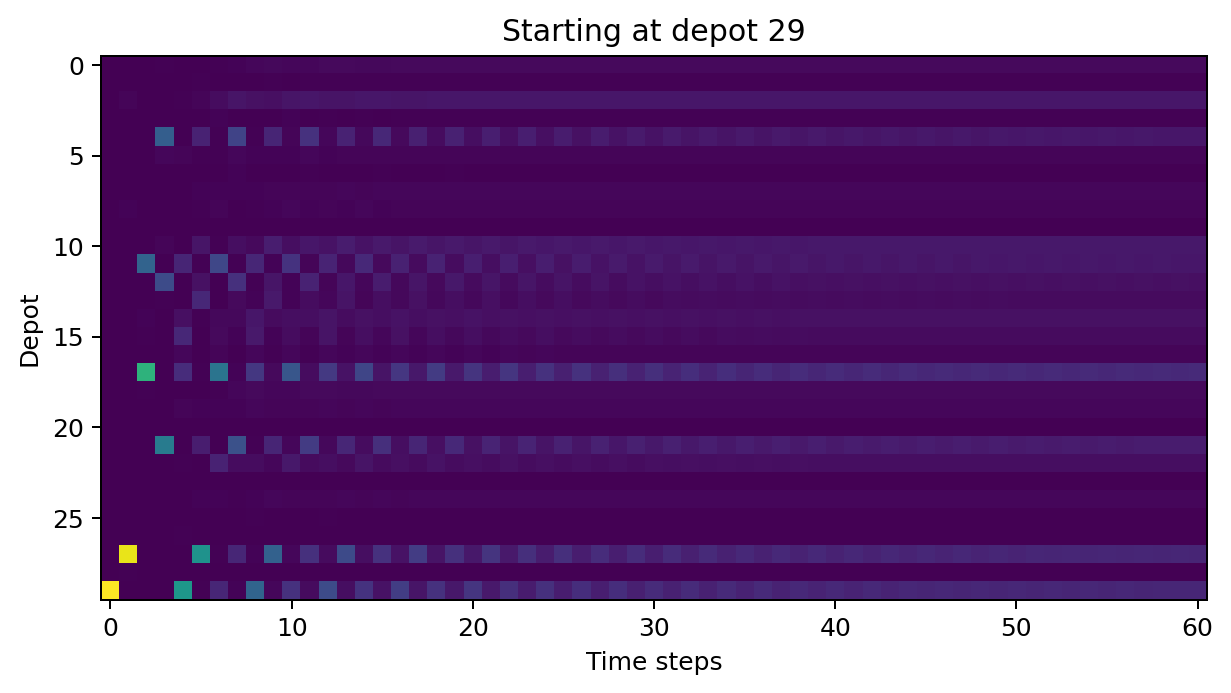
\includegraphics[scale=0.4]{src/3.26 Start at 29.png}
        \caption{The evolution of package locations over time, starting at depot 29.}
    \end{figure}
    \noindent No matter which depot we start from, the packages end up about the same configuration. This is a steady state- in terms of adjacency matrix, this is an eigenvector.

    Matrices represent linear transformations, which involves rotation and/or scaling vectors. But, there are some vectors that do not get rotated by a linear transformation- they only get scaled. Such vectors are called eigenvalues, and the scaling factor is an eigenvalue.

    We can find the leading (biggest) eigenvalue by power iteration. Given a vector $\mathbf{x}$ and a matrix $A$, and a number of iterations $n$, the power iteration computes $A^n \mathbf{x}$, but normalising at each multiplication, i.e. $\mathbf{x}_0 = \mathbf{x}$, and
    \[\mathbf{x}_{i+1} = \frac{A \mathbf{x}_i}{\lVert A \mathbf{x}_i \rVert_{\infty}}.\]
    By normalising, we ensure the value doesn't increase to $\infty$ or decrease to $0$. We can normalise using any norm- the infinity norm is the most efficient/most commonly used.

    Regardless of our choice of $\mathbf{x}$, the vector we find after power iteration is unique (up to sign)- this is true for most square matrices. The resulting vector is the leading eigenvector. It has to just scale the vector (and not rotate) since we are always normalising- the scale effect is remove. We can use the relation $A \mathbf{x} = \lambda \mathbf{x}$ to compute the leading eigenvalue. Here, $\lambda$ is the (leading) eigenvalue, and $\mathbf{x}$ is the (leading) eigenvector.

    For an $n \times n$ matrix, there are $n$ eigenvalues and $n$ corresponding eigenvectors. The eigenvectors are orthogonal, i.e. the dot product of any two eigenvectors is 0. Power iteration is much faster than the function \texttt{np.linalg.eig} when computing the leading eigenvalue/eigenvector for large matrices.

    For an $n \times n$ matrix $A$, an eigenvalue $\lambda$ is a real number and the corresponding eigenvector $\mathbf{x}$ is a vector in $\mathbb{R}^n$ such that $A \mathbf{x} = \lambda \mathbf{x}$. A matrix has a unique set of eigenvalues, but not a unique set of eigenvectors (e.g. the negative of an eigenvector is still an eigenvector). Problems that can be solved using eigenvectors and eigenvalues are called eigenproblems.

    Using undirected graphs (i.e. symmetric matrices) will ensure that all the eigenvalues/eigenvectors are real. If none of the eigenvalues were real for some matrix, there would be no steady state- it will oscillate.

    Now, we consider the example of packages going through depots again. Let $A$ be the adjacency matrix for the weighted graph. We can show the eigenvectors of $A$, scaled by the eigenvalue:
    \begin{figure}[H]
        \centering
        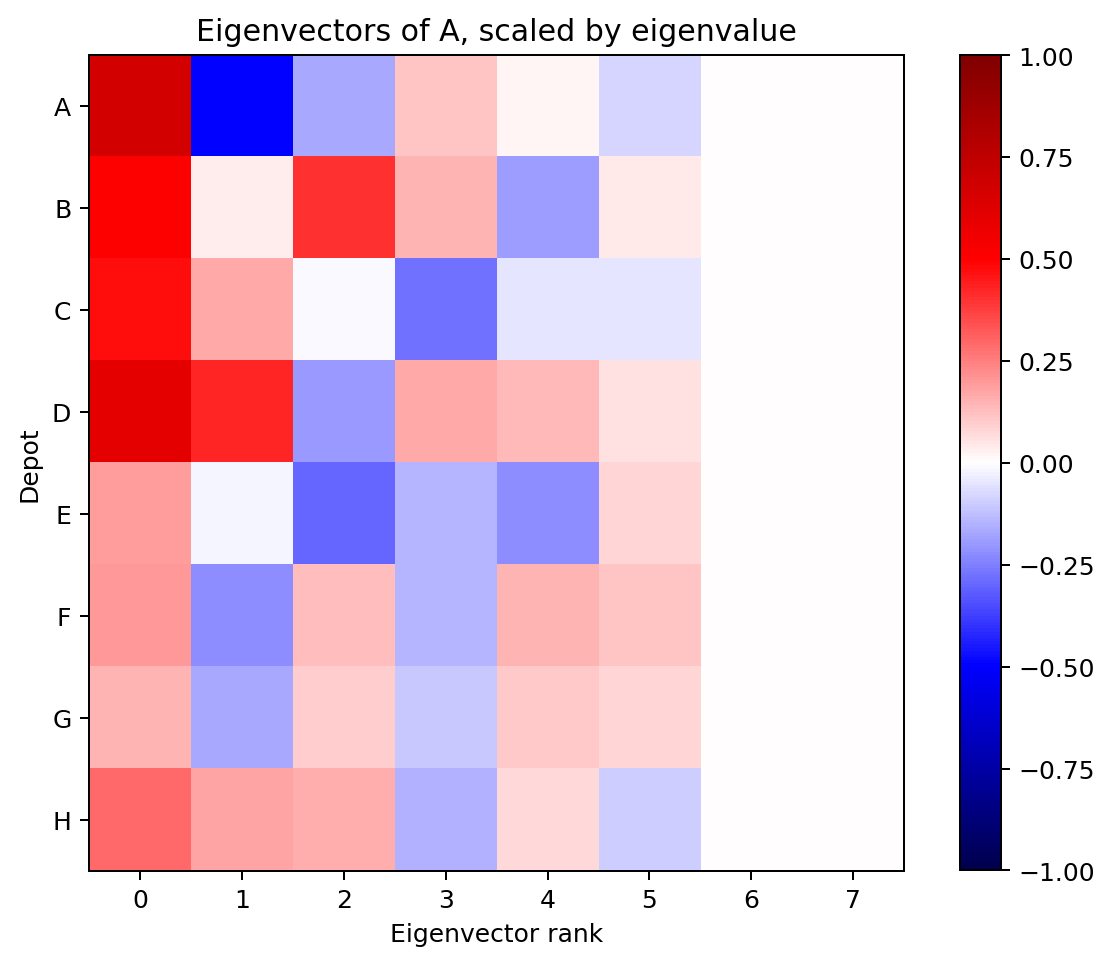
\includegraphics[scale=0.4]{src/3.27 Eigenvectors scaled by eigenvalue.png}
        \caption{The eigenvectors of the adjacency matrix, scaled by eigenvalue.}
    \end{figure}
    The leading eigenvector says where the packages will end up in the long run- they will end up mostly in depot A, D, B, C and H. Smaller eigenvalues represent the routes less commonly used, while larger eigenvalues are the dominant routes taken by packages.

    From the eigendata, we can construct the eigenspectrum- this is just the eigenvalues ordered by the magnitude (biggest one first). This ranks the eigenvalues in order of importance.
    \begin{figure}[H]
        \centering
        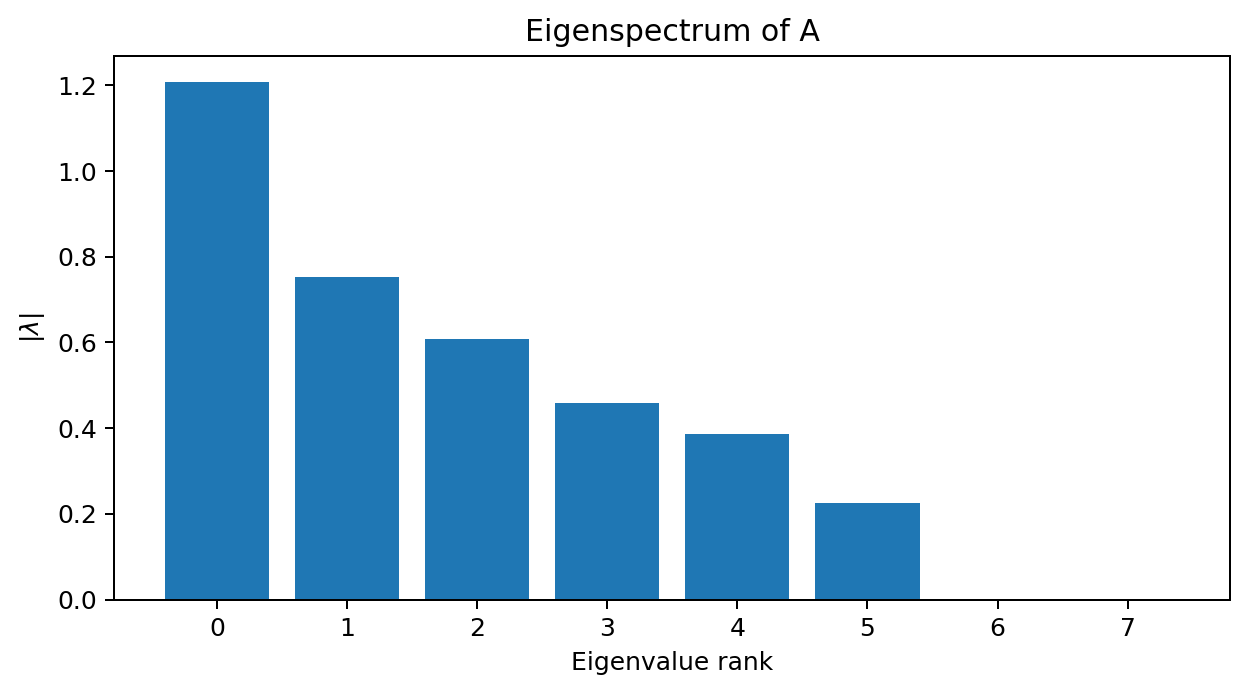
\includegraphics[scale=0.4]{src/3.28 Eigenspectrum.png}
        \caption{The eigenspectrum of the matrix.}
    \end{figure}
    
    \section{Issues in eigendecomposition}
    The function \texttt{np.linalg.eig} is numerically unstable because of rounding errors due to limitations in floating point representations. Nonetheless, it is pretty good most of the time. A more stable algorithm for real, symmetric matrices is \texttt{np.linalg.eigh}. Typically, there is not a big difference in eigenvalues/eigenvectors if they are big. However, there could be a big difference in eigenvalues/eigenvectors when the values are very small. However, \texttt{np.linalg.eigh} is typically better.

    \section{Principal component analysis}
    We know that the covariance matrix gives us insight into correlations between variables in the dataset. We can plot a representation of the covariance matrix as an ellipse which aligns with the distribution of the data points. Uncorrelated data looks close to a circle, while strong correlations correspond to a long, thin ellipse. The eigenvectors of the covariance matrix, scaled by the eigenvalue, from the principal axes of the ellipse.
    \begin{figure}[H]
        \centering
        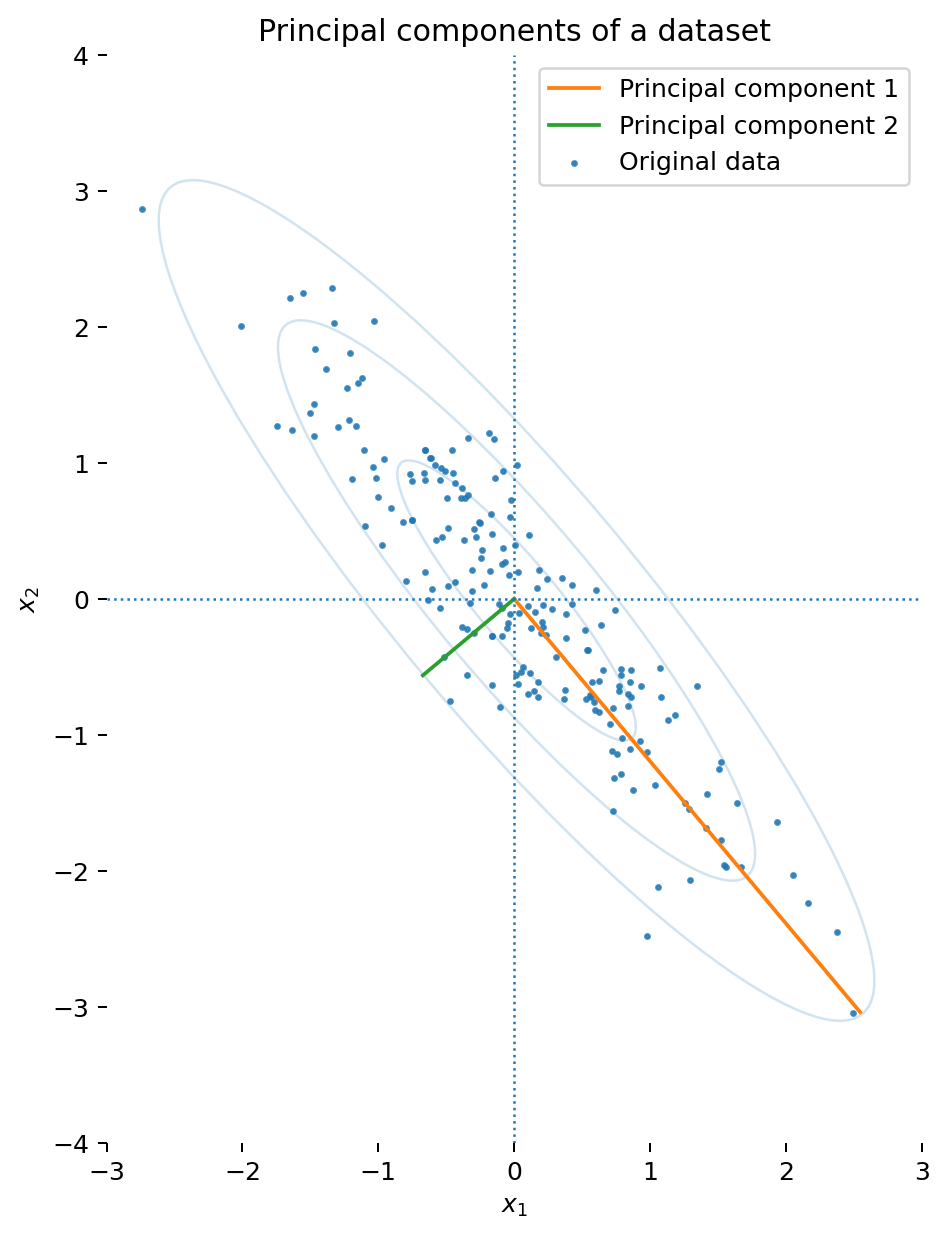
\includegraphics[scale=0.6]{src/3.29 Principal components of a dataset.png}
        \caption{The principal components of a dataset.}
    \end{figure}
    We have decomposed the covariance matrix into eigenvectors and eigenvalues. It is also possible to recompose the covariance matrix using the eigenvalues and eigenvectors. This is given by $\Sigma = Q \Lambda Q^T$, where $\Sigma$ is the covariance matrix, $Q$ is a matrix of unit eigenvectors (same as \texttt{np.linalg.eig}) and $\Lambda$ is a diagonal matrix of eigenvalues.

    If our dataset has a lot of dimensions, then $\Sigma$ is going to be very large. In that case, we would want to approximate the covariance matrix by only storing the first few principal components. Keeping the larger principal components means that we keep most of the data.

    Matrix approximation allows us to simplify the transformation and compress matrices. The approximation depends on the eigenspectrum:
    \begin{itemize}
        \item If we have one big eigenvalue and all the others are much smaller, we can just take the first eigenvalue to approximate the dataset.
        \item Instead, if all the eigenvalues have similar magnitude, then we will not be able to transform the data easily.
    \end{itemize}
    We can also reduce the dimension of the data by projecting it onto few principal components (of the covariance matrix). This involves multiplying the dataset matrix by each component, and saving the projected data into another matrix. We can project the data above to the 1st principal component:
    \begin{figure}[H]
        \centering
        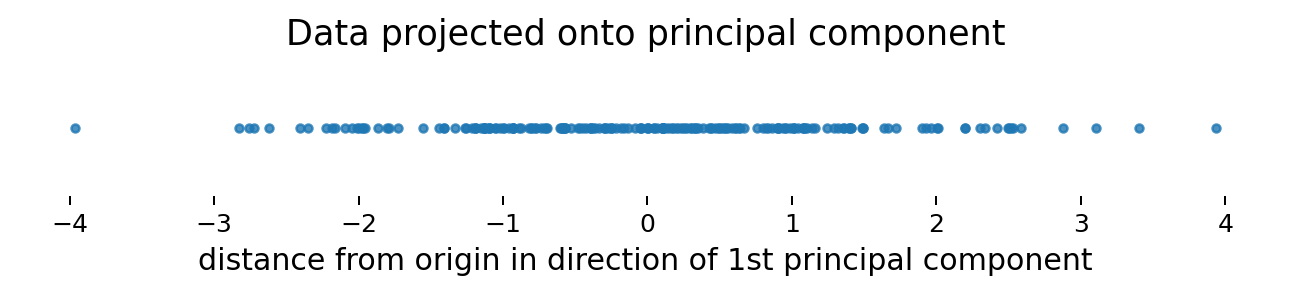
\includegraphics[scale=0.6]{src/3.30 Data projected onto principal component.png}
        \caption{Projecting the data onto the first principal component.}
    \end{figure}
    Here, we reduced the 2D data into 1D. It is more common to reduce high-dimensional data into 2D. It is much easier to visualise in 2D- it allows us to find structure in data (e.g. clusters).

    Matrix decomposition has applications everywhere. Eigendecomposition can be used if we have a system modelled as a linear transformation (i.e. a linear map $\mathbb{R}^n \to \mathbb{R}^n$). It lets us predict behaviour over different time scales, e.g.
    \begin{itemize}
        \item finding modes/resonances of a system;
        \item predicting behaviour of feedback control systems;
        \item partitioning graph and cluster data (spectral clustering);
        \item predicting graph flows;
        \item performing Principal Component Analysis on high-dimensional data sets for exploratory data analysis, 2D visualisation or data compression.
    \end{itemize}

    \section{Determinant, trace and definiteness}
    \subsection{Trace and determinant}
    The trace of a matrix is the sum of the diagonal entries. It is also the sum of the eigenvalues. It can be thought of as the perimeter of the parallelotope of a unit cube transformed by the matrix.

    The determinant of a matrix can be thought of as the area of the parallelotope of a unit cube transformed by the matrix. It is the product of the eigenvalues. In particular, if any eigenvalue is 0, then the determinant is 0. This means that the transformation collapses at least one dimension. Therefore, this transformation cannot be reversed; information has been lost.

    \subsection{Definiteness}
    There are also 4 other ways of classifying a matrix:
    \begin{itemize}
        \item if every eigenvalue of a matrix is strictly positive, then the matrix is positive-definite;
        \item if every eigenvalue of a matrix is non-negative, then the matrix is positive semi-definite;
        \item if every eigenvalue of a matrix is strictly engative, then the matrix is negative-definite;
        \item if every eigenvalue of a matrix is non-positive, then the matrix is negative semi-definite.
    \end{itemize}
    A positive definite matrix $A$ satisfies $\mathbf{x}^T A \mathbf{x} > 0$ for all vectors $\mathbf{x}$ in $\mathbb{R}^n$. We know that $\mathbf{x}^T A \mathbf{x} = |\mathbf{x}| |A \mathbf{x}| \cos \theta$, so $A$ must rotate a vector by at most $90^{\circ}$.

    We can conclude many properties about the transformation corresponding to a matrix using its eigenspectrum:
    \begin{itemize}
        \item if a matrix has one or more zero eigenvalues, the transform it performs is one that collapses one or more dimensions in a vector space. This type of operation is irreversible, and this tells us that $A$ is singular- more on that in a moment.
        \item Eigenvectors corresponding to larger (absolute) eigenvalues are more ``important''; they represents directions in which data will get stretched by the most.
        \item If the eigenspectrum is nearly flat (i.e. eigenvalues all have similar values), then $A$ represents a transform that stretches vectors almost equally in all directions (like transforming a sphere to another sphere).
        \item If the eigenspectrum has few large eigenvalues and lots of small ones, then vectors will get stretched along a few directions, but shrink away to nothing along others (like transforming a sphere to a long, skinny ellipse).
    \end{itemize}

    \section{Inversion}
    For some $n \times n$ matrices $A$, there exists an inverse matrix $A^{-1}$ such that:
    \begin{itemize}
        \item $A^{-1}(A \mathbf{x}) = \mathbf{x}$,
        \item $A^{-1}A = I$,
        \item $(A^{-1})^{-1} = A$.
    \end{itemize}
    Therefore, $A^{-1}$ has the effect of undoing $A$. 
    Also, for square matrices $A, B$, $(AB)^{-1} = B^{-1} A^{-1}$. We can invert a square matrix using \texttt{np.linalg.inv}. Inversion can undo a transformation as long as no information was lost as part of the transformation.

    We illustrate inversion with an example. Let $A$ be a $2 \times 2$ matrix that rotates the 2D plane by $30^{\circ}$:
    \begin{figure}[H]
        \centering
        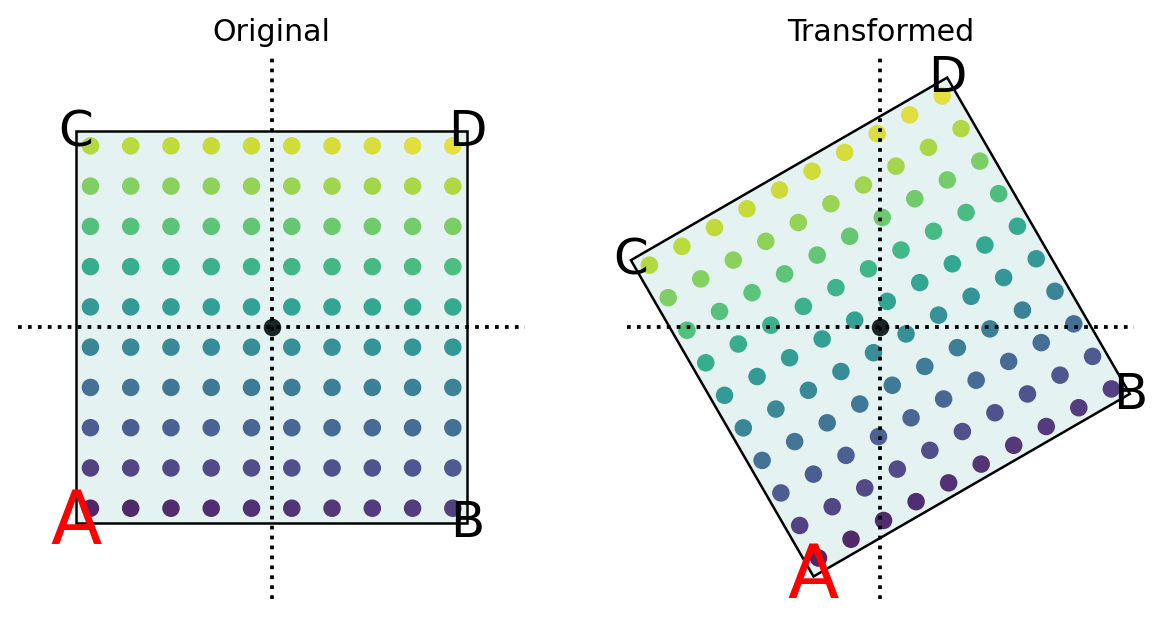
\includegraphics[scale=0.4]{src/3.31 Inverse 2D transform Original.png}
        \caption{The $2 \times 2$ matrix that transforms the 2D plane.}
    \end{figure}
    \noindent Its inverse matrix gives the following transformation.
    \begin{figure}[H]
        \centering
        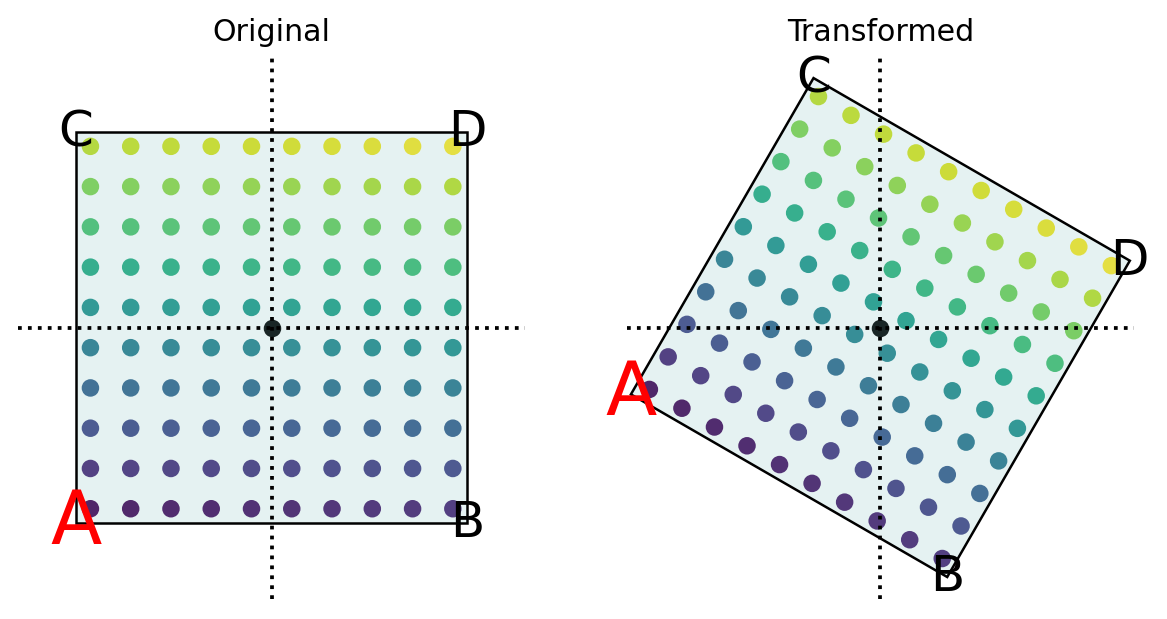
\includegraphics[scale=0.4]{src/3.32 Inverse 2D transform Inverse.png}
        \caption{The inverse transformation of the transformation above.}
    \end{figure}
    A condition for a square matrix for having an inverse is for none of the eigenvalues to be 0. It is equivalent to saying that the determinant is non-zero. A matrix being invertible is equivalent to the function represented by the matrix being bijective. An $n \times m$ matrix which is non-square maps vectors of dimension $m$ to dimension $n$. This means that the transformation collapses or creates dimensions. Such a transformation is not uniquely reversible- it is not bijective. 
    
    A matrix that is not invertible is called singular. An invertible matrix is called non-singular. The figure below shows a singular transformation of the 2D plane.
    \begin{figure}[H]
        \centering
        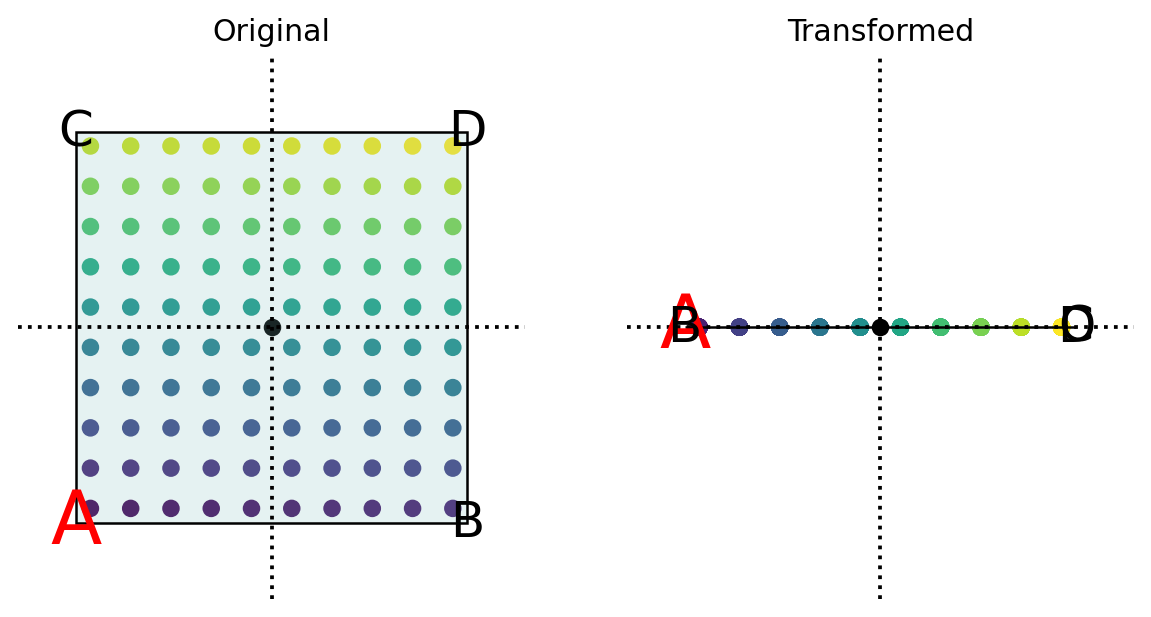
\includegraphics[scale=0.4]{src/3.33 2D singular transform.png}
        \caption{A transformation of the 2D plane by a singular matrix.}
    \end{figure}
    Since matrix operations involve lots of floating point operations, there are many operations for rounding errors to accumulate. Inversion is particularly hard to compute in a stable form directly. Moreover, many matrices that theoretically could be inverted cannot be inverted using floating point representation.

    Nonetheless:
    \begin{itemize}
        \item if a matrix is orthogonal (i.e. rows and columns are all orthogonal unit vectors), then its inverse is its transpose- this can be computed in $O(1)$ time;
        \item if a matrix is diagonal, then its inverse is just another diagonal matrix with reciprocal of the original diagonal entries- this can be computed in $O(n)$ time;
        \item if a matrix is positive-definite, then its inverse can be computed in $O(n^2)$ time using Cholesky decomposition;
        \item if a matrix is triangular, then its inverse can be computed in $O(n^2)$ using elimination algorithms.
    \end{itemize}
    An orthogonal matrix has eigenvalues $1$ or $-1$. An orthogonal matrix corresponds to a matrix that purely rotates the plane. For example, rotation by $30^{\circ}$ corresponds to an orthogonal matrix. A diagonal matrix corresponds to one that only scales a matrix.

    In general, the inverse of a sparse matrix is not sparse. This means that sparse matrix algorithms virtually never involve a direct inverse, since a sparse matrix could be easily be $10^6 \times 10^6$, but with maybe only a few million non-zero entries, and might be stored in a few dozen megabytes. The inverse form would have $10^{12}$ entries and would require a terabyte or more to store.

    \section{Solving linear systems}
    We can use the inverse matrix to take one step to the past. For instance, if $A$ corresponds to one day forward, $A^{-1}$ corresponds to one day backwards. To go $n$ days backwards, we can compute $(A^{-1})^n$. However, inversion is highly problematic from a numerical point of view, and roundoff error will lead to severely distorted results with repeated negative powers of a matrix.

    A matrix corresponds to a system of equations. For instance, the matrix 
    \[\begin{bmatrix}
        0.5 & 1.0 & 2.0 \\
        1.0 & 0.5 & 0.0 \\
        0.6 & 1.1 & -0.3
    \end{bmatrix}\]
    corresponds to the system of equations 
    \begin{align*}
        y_1 &= 0.5x_1 + 1.0x_2 + 2.0x_3 \\
        y_2 &= 1.0x_1 + 0.5x_2 + 0.0x_3 \\
        y_3 &= 0.6x_1 + 1.1x_2 - 0.3x_3.
    \end{align*}
    We can use the inverse of a matrix to find the solution. A matrix corresponds to $A \mathbf{x} = \mathbf{y}$, so the solution to the system is $\mathbf{x} = A^{-1} \mathbf{y}$. As this only works for square matrices, $\mathbf{x}$ and $\mathbf{y}$ must have the same dimension. An alternative approach in solving these linear equations is to find $\mathbf{x}$ such that $\lVert A \mathbf{x} - \mathbf{y} \rVert$.
    
    \section{The SVD}
    Like eigendecomposition can be used to decompose square matrices, there is a generalisation- singular value decomposition (SVD). Given $n \times m$ matrix $A$, we can write
    \[A = U \Sigma V^T,\]
    where:
    \begin{itemize}
        \item $U$ is an $m \times m$ square unitary matrix, whose columns contain the left singular vectors;
        \item $V$ is an $n \times n$ square unitary matrix, whose columns contain the right singular vectors;
        \item $\Sigma$ is an $n \times m$ matrix, whose diagonal contains the singular values.
    \end{itemize}
    A unitary matrix is one whose conjugate tranpose is equal to its inverse. If $A$ is real, then $U$ and $V$ will be orthogonal.

    The diagonal matrix $\Sigma$ is the set of singular values, which are closely related to the eigenvalues, but are not quite the same thing (except for special cases like $A$ is a positive semi-definite symmetric matrix). The singular values are always positive real numbers.

    The SVD is the same as:
    \begin{itemize}
        \item taking the eigenvectors of $A^T A$ to get $U$;
        \item takng the square root of the absolute value of the eigenvalues $\lambda_i$ of $A^T A$ to get $\Sigma_i = \sqrt{|\lambda_i|}$;
        \item taking the eigenvectors of $AA^T$ to get $V^T$.
    \end{itemize}
    If $A$ is symmetric, positive semi-definite matrix, then the eigenvectors of the columns of $U$ or the columns of $V$. The eigenvalues are in $\Sigma$.

    So, SVD can convert any matrix into a product of 3 matrices, $U$, $\Sigma$ and $V$, where
    \begin{itemize}
        \item $U$ is orthogonal, i.e. it is purely rotational;
        \item $\Sigma$ is diagonal, i.e. it is purely scaling; and
        \item $V$ is orthogonal, i.e. it is purely rotational.
    \end{itemize}

    \section{Using the SVD for fractional powers}
    We can use the SVD to compute fractional powers of a matrix. For an $n \times m$ matrix $A$, $A^k = V \Sigma^k U^T$ (and if $A$ is symmetric, then $A^k = U \Sigma^k V^T$ is also the same thing). We can also use the SVD to compute the inverse of a square matrix: $A^{-1} = V \Sigma^{-1} U^T$. This can be computed in $O(n)$ time since $\Sigma^{-1}$ can be computed by reciprocating the diagonal entries in $\Sigma$.

    Moreover, we can compute the pseudo-inverse of a matrix, even if it isn't a square/inverse. It is given by the same formula $A^{+} = V \Sigma^{-1} U^T$. This allows us to invert (some) non-square matrices. We pad $\Sigma$ with zeroes to invert it. The function \texttt{np.linalg.pinv} does this computation. It is possible that the problem doesn't have an exact solution- the pseudo-inverse function tries to minimise $\lVert A \mathbf{x} - \mathbf{y} \rVert_2$.

    Assume that we have 2 datasets, one consisting of $\mathbf{x}$ values and the other with $\mathbf{y}$ values, in matrices $X$ and $Y$ respectively. We want to fit a line to this dataset to predict $\mathbf{y}$ values, using $\mathbf{y} = A \mathbf{x}$, or lots of $\mathbf{y}$ values at the same time, using $Y = AX$. The equation of the line/plane is given in $A$, i.e. $\mathbf{x} = A^+ \mathbf{y}$. In general, we have $A = X^+ Y$. We can use this formula to fit a line/plane through the dataset, even when we have many more points than the number of dimensions required to specify the line/plane. A system of equations where there are more inputs than outputs is called ``overdetermined''.
    
    \section{Rank and condition}
    \subsection{Rank of a matrix}
    The rank of a matrix is the number of non-zero singular values. If the number of non-zero singular values is equal to the size of the matrix, then the matrix is full rank. A full rank matrix has a non-zero determinant and will be invertible. The rank tells us how many dimensions of the parallelotope that the transform represents will have. If a matrix does not have full rank, it is singular (non-invertible) and has deficient rank. If the number of non-zero singular values is much less than the size of the matrix, the matrix is low rank.

    For example, a $4 \times 4$ matrix with rank 2 will take vectors in $\mathbb{R}^4$ and output vectors in $\mathbb{R}^2$ subspace (a plane) of $\mathbb{R}^4$. The orientation of that plane will be given by the first two eigenvectors of the matrix.

    \subsection{Condition of a matrix}
    The condition number of a matrix is the ratio of the largest singular value to the smallest. This is only defined for full rank matrices. The condition number measures how sensitive inversion of the matrix is to small changes. A matrix with a small condition number is called well-conditioned and is unlikely to cause numerical issues. A matrix with a large condition number is ill-conditioned, and numerical issues are likely to be significant.

    Inverting an ill-conditioned matrix will not be very accurate due to the floating point roundoff errors. We can think of rank as measuring ``how singular'' the matrix is, i.e. how many dimensions are lost in the transformation. We can think of the condition number as measuring how close a non-singular matrix is to being singular. A matrix which is nearly singular may become effectively singular due to floating point roundoff errors.

    \section{Whitening a dataset}
    Whitening removes all linear correlations within the data. Given a matrix $X$, the whitened matrix $X^w$ is given by $X^w = (X - \mu) \Sigma^{-1/2}$, where $\mu$ is the mean row vector (containing the mean of each column), and $\Sigma$ is the covariance matrix.

    By subtracting the mean, the data gets centered at the origin (zero mean). By multiplying it with $\Sigma^{-1/2}$, it essentially divides by the standard deviation and normalises the spread of data in each column (squashes data so it has unit covariance).
    \begin{figure}[H]
        \centering
        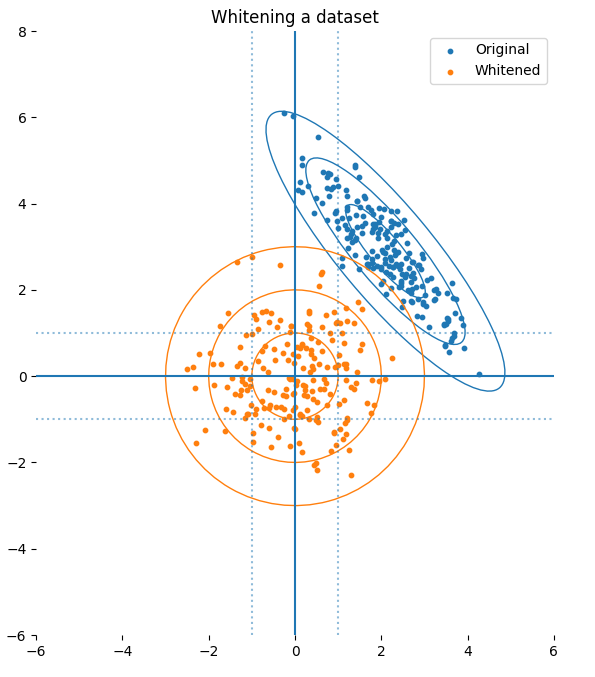
\includegraphics[scale=0.5]{src/3.34 Whitening dataset.png}
        \caption{Whitening a dataset by centering the mean and removing variation.}
    \end{figure}
\end{document}
